\ifx\allfiles\undefined
\documentclass[a4paper,fleqn]{cas-sc}
% \documentclass[a4paper,fleqn,longmktitle]{cas-sc}
\usepackage{rotating}
\usepackage{appendix}
\usepackage{graphicx}
\usepackage{caption}
\usepackage{tabularray}
\usepackage[authoryear]{natbib}
\usepackage{float}
\usepackage{tabularx}
\usepackage{makecell}
\usepackage{amsmath}
\usepackage{mathtools}
\usepackage{color}
\usepackage{booktabs}
\usepackage{array}
\usepackage{pdflscape}
\usepackage{longtable}
\let\printorcid\relax
\definecolor{customblue}{rgb}{0, 0.501, 0.675}
\hypersetup{
  linkcolor = customblue,  % 使用自定义颜色 customblue
  citecolor = customblue,  % 可以为引用也设置同样的颜色或另外选择
  urlcolor = customblue    % 设置外部链接颜色
}
%%%Author macros
\def\tsc#1{\csdef{#1}{\textsc{\lowercase{#1}}\xspace}}
\tsc{WGM}
\tsc{QE}
%%%

% Uncomment and use as if needed
%\newtheorem{theorem}{Theorem}
%\newtheorem{lemma}[theorem]{Lemma}
%\newdefinition{rmk}{Remark}
%\newproof{pf}{Proof}
%\newproof{pot}{Proof of Theorem \ref{thm}}
\captionsetup[figure]{labelfont={bf},name={Fig. },labelsep=period}
% \captionsetup[table]{ labelsep=newline,singlelinecheck=true }
\captionsetup[table]{labelfont={bf},labelsep=period,name={Table}} 
\captionsetup[longtblr]{font=bf, labelsep=period, justification=raggedright} % longtblr 专用设置
\begin{document}
\let\WriteBookmarks\relax
\def\floatpagepagefraction{1}
\def\textpagefraction{. 001}

% Short title
\shorttitle{} 

% Short author
\shortauthors{ {Zhou et al. }}

% Main title of the paper
\title [mode = title]{Twenty-five years of the intelligent driver model: Bibliometric Analysis and Systematic Review with Critical Reflections}
% Author Information
\author[label1,label2]{Shirui Zhou}
\ead{shiruizhou@tju.edu.cn}

\author[label4]{H. M. Zhang}
\ead{hmzhang@ucdavis.edu.cn}

\author[label3]{Shiteng Zheng}
\ead{stzheng1@bjtu.edu.cn}

% \author[label4]{Martin Treiber}
% \ead{martin@mtreiber.de}

\author[label1,label2]{Junfang Tian}
\cormark[1]
\ead{jftian@tju.edu.cn}

\author[label3]{Rui Jiang}
\cormark[1]
\ead{jiangrui@bjtu.edu.cn}



\affiliation[label1]{organization={Institute of Systems Engineering, College of Management and Economics, Tianjin University},
addressline={No. 92 Weijin Road},
city={Nankai District},
postcode={300072},
state={Tianjin},
country={China}}
\affiliation[label2]{organization={Laboratory of Computation and Analytics of Complex Management Systems (CACMS),Tianjin University},
addressline={No. 92 Weijin Road},
city={Nankai District},
postcode={300072},
state={Tianjin},
country={China}}
\affiliation[label4]{organization={Department of Civil and Environmental Engineering, University of California Davis},
            addressline={2001 Ghausi Hall Davis},
            city={Davis},
            postcode={95616},
            state={California},
            country={United States}}   
\affiliation[label3]{organization={School of Systems Science, Beijing Jiaotong University},
addressline={No. 3 Shangyuancun},
city={Haidian District},
postcode={100044},
state={Beijing},
country={China}}
    
% \affiliation[label4]{organization={Institute for Transport and Economics, Dresden University of Technology},
% addressline={Würzburger Str. 35},
% city={Dresden},
% postcode={D-01062},
% state={Saxony},
% country={Germany}}
% Corresponding author text
\cortext[1]{Corresponding author. }

% For a title note without a number/mark
% \nonumnote{}

% Here goes the abstract
\begin{abstract}
The Intelligent Driver Model (IDM), proposed by \cite{treiberCongestedTrafficStatesEmpirical2000}, is recognized as a landmark in traffic flow modeling due to its simplicity and effectiveness in capturing traffic dynamics. Over the past quarter century, IDM has evolved into a foundational tool in traffic flow theory and intelligent transportation systems. Its adaptability and robustness have not only advanced the understanding of car-following behavior but also facilitated its adoption in emerging fields such as autonomous driving.This paper aims to provide a 25th anniversary bibliometric analysis of IDM-related research. A bibliometric approach is employed to identify the distribution of journal publications, influential papers, key contributors, and leading topics over the past 25 years. The literature is classified based on recurring themes, including original IDM overview, theoretical applications, practical applications, and extensions of IDM. For each theme, typical research developed to date is surveyed, and potential directions for future studies are discussed. 
\end{abstract}

% Keywords
% Each keyword is seperated by \sep
\begin{keywords}
Intelligent driver model\sep Bibliometric analysis\sep Driving behavior modeling\sep trajectory
\end{keywords}

\maketitle
% Main text
\section{Introduction}

Accurate modeling and understanding the individual vehicle behavior are crucial for analyzing and predicting traffic flow dynamics and related engineering application. Car following models are fundamental to this task, as they detail how drivers adjust their vehicle speed in response to the vehicle ahead. These models facilitate the simulation of diverse traffic conditions and reveal the complex relationships between driver behavior and traffic stability. By capturing vehicle interactions at a micro level, car following models provide essential theoretical support for the design of intelligent transportation systems and the optimization of traffic management strategies, such as the Intelligent Driver Model (IDM, \cite{treiberCongestedTrafficStatesEmpirical2000}), the Optimal Velocity Model (OVM, \cite{bandoDynamicalModelTrafficCongestion1995a}), the Full Velocity Difference Model (FVDM, \cite{jiangFullVelocityDifferenceModel2001a}), Newell's model \citep{newellSimplifiedCarfollowingTheoryLower2002}, Gipps' model \citep{gippsBehaviouralCarfollowingModelComputer1981a}, GM model \citep{chandlerTrafficDynamicsStudiesCar1958}, GHR model \citep{gazisNonlinearFollowLeaderModelsTraffic1961} and Wiedemann model\citep{wiedemann1992microscopic}. 

Among these models, IDM stands out as one of the most widely used microscopic models for replicating driving behavior in traffic flow. This model conceptualizes each vehicle as an intelligent agent, adjusting its acceleration based on nonlinear interactions with the vehicle ahead, considering factors such as distance, relative velocity, and desired speed. It effectively captures various traffic states, including free flow and congestion, as well as complex traffic phenomena like stop-and-go waves and hysteresis effects. The IDM's effectiveness and computational efficiency in modeling these dynamics have established it as a benchmark in traffic flow modeling. The formulation of IDM is as follows:

\begin{equation}
a_n(t) = a \left[ 1 - \left( \frac{v_n(t)}{v_0} \right)^4 - \left( \frac{s^*_n(t)}{s_n(t)} \right)^2 \right]
\label{equ:IDM1}
\end{equation}
where \( a_n(t) \) represents the vehicle's acceleration, \( a \) is the maximum acceleration, \( v_n(t) \) is the current velocity, \( v_0 \) is the desired velocity, \( s_n(t) \) is the actual spacing, and \( s^*_n(t) \) is the desired dynamic spacing. The desired spacing \( s^*_n(t) \) is defined as:

\begin{equation}
s^*_n(t) = s_0 + \max \left( T v_n(t) + \frac{v_n(t) \Delta v_n(t)}{2\sqrt{ab}}, 0 \right)
\label{equ:IDM2}
\end{equation}

where \( s_0 \) is the minimum spacing, \( T \) is the time gap, \( \Delta v_n(t) = v_n(t) - v_{n-1}(t) \) is the velocity difference to the preceding vehicle n-1, and \( b \) is the comfortable deceleration. The model captures critical driving behaviors by decreasing acceleration as the vehicle approaches its desired speed and ensuring safety through dynamic spacing. 


IDM can effectively simulate realistic traffic dynamics and provides insights into complex traffic phenomena, making it an instrumental tool for traffic flow analysis over the past 25 years. As a foundational model, IDM has significantly enhanced the understanding and representation of driver behavior, facilitating complex analyses such as the derivation of fundamental diagrams and comprehensive assessments of traffic flow stability. In the realm of calibration, IDM has clarified the interaction between driving states and calibration parameters, spurring the development of advanced calibration algorithms and comprehensive frameworks. Its practical applications are extensive, seamlessly integrating into simulation platforms like SUMO and playing a pivotal role in designing vehicle control algorithms for autonomous driving scenarios. These advancements underscore IDM's influence in traditional traffic flow modeling theory and its practical application in modern intelligent and connected transportation systems, solidifying its status as an indispensable tool for advancing contemporary transportation systems.

To date, numerous studies have explored the IDM and its variations, highlighting its increasingly significance in traffic flow modeling. These studies span decades, focusing on specific aspects of application and development of IDM. Given the rapid advancements in autonomous driving and connected vehicle technologies, it is timely to conduct a comprehensive review of evolution and impact of IDM. This paper aims to provide a systematic evaluation that sets it apart from previous reviews. First, it is crucial to examine the extensive body of literature concerning IDM to appreciate its role in advancing traffic modeling.This involves reviewing all relevant topics published in journals, but papers that simply cite IDM without analyzing or applying it are excluded due to the large number of publications citing IDM. Second, a bibliometric analysis is employed to trace the scholarly impact of IDM, mapping the network of publications, influential papers, and leading authors in the field. Utilizing tools such as VOSviewer, this approach allows for a clear visualization of influence of IDM across various research domains. Third, based on this analysis, we present a critical review of existing studies and identify current research gaps and opportunities. The insights gained from these analyses underscore pivotal role of IDM in shaping both theoretical and practical aspects of modern traffic systems.

The rest of the paper is structured as follows: Section 2 presents a bibliometric analysis. Section 3 organizes and examines the relevant literature. Section 4 explores possible avenues for future research. Finally, Section 5 provides the conclusion.


\begin{figure}[H]
    \centering
    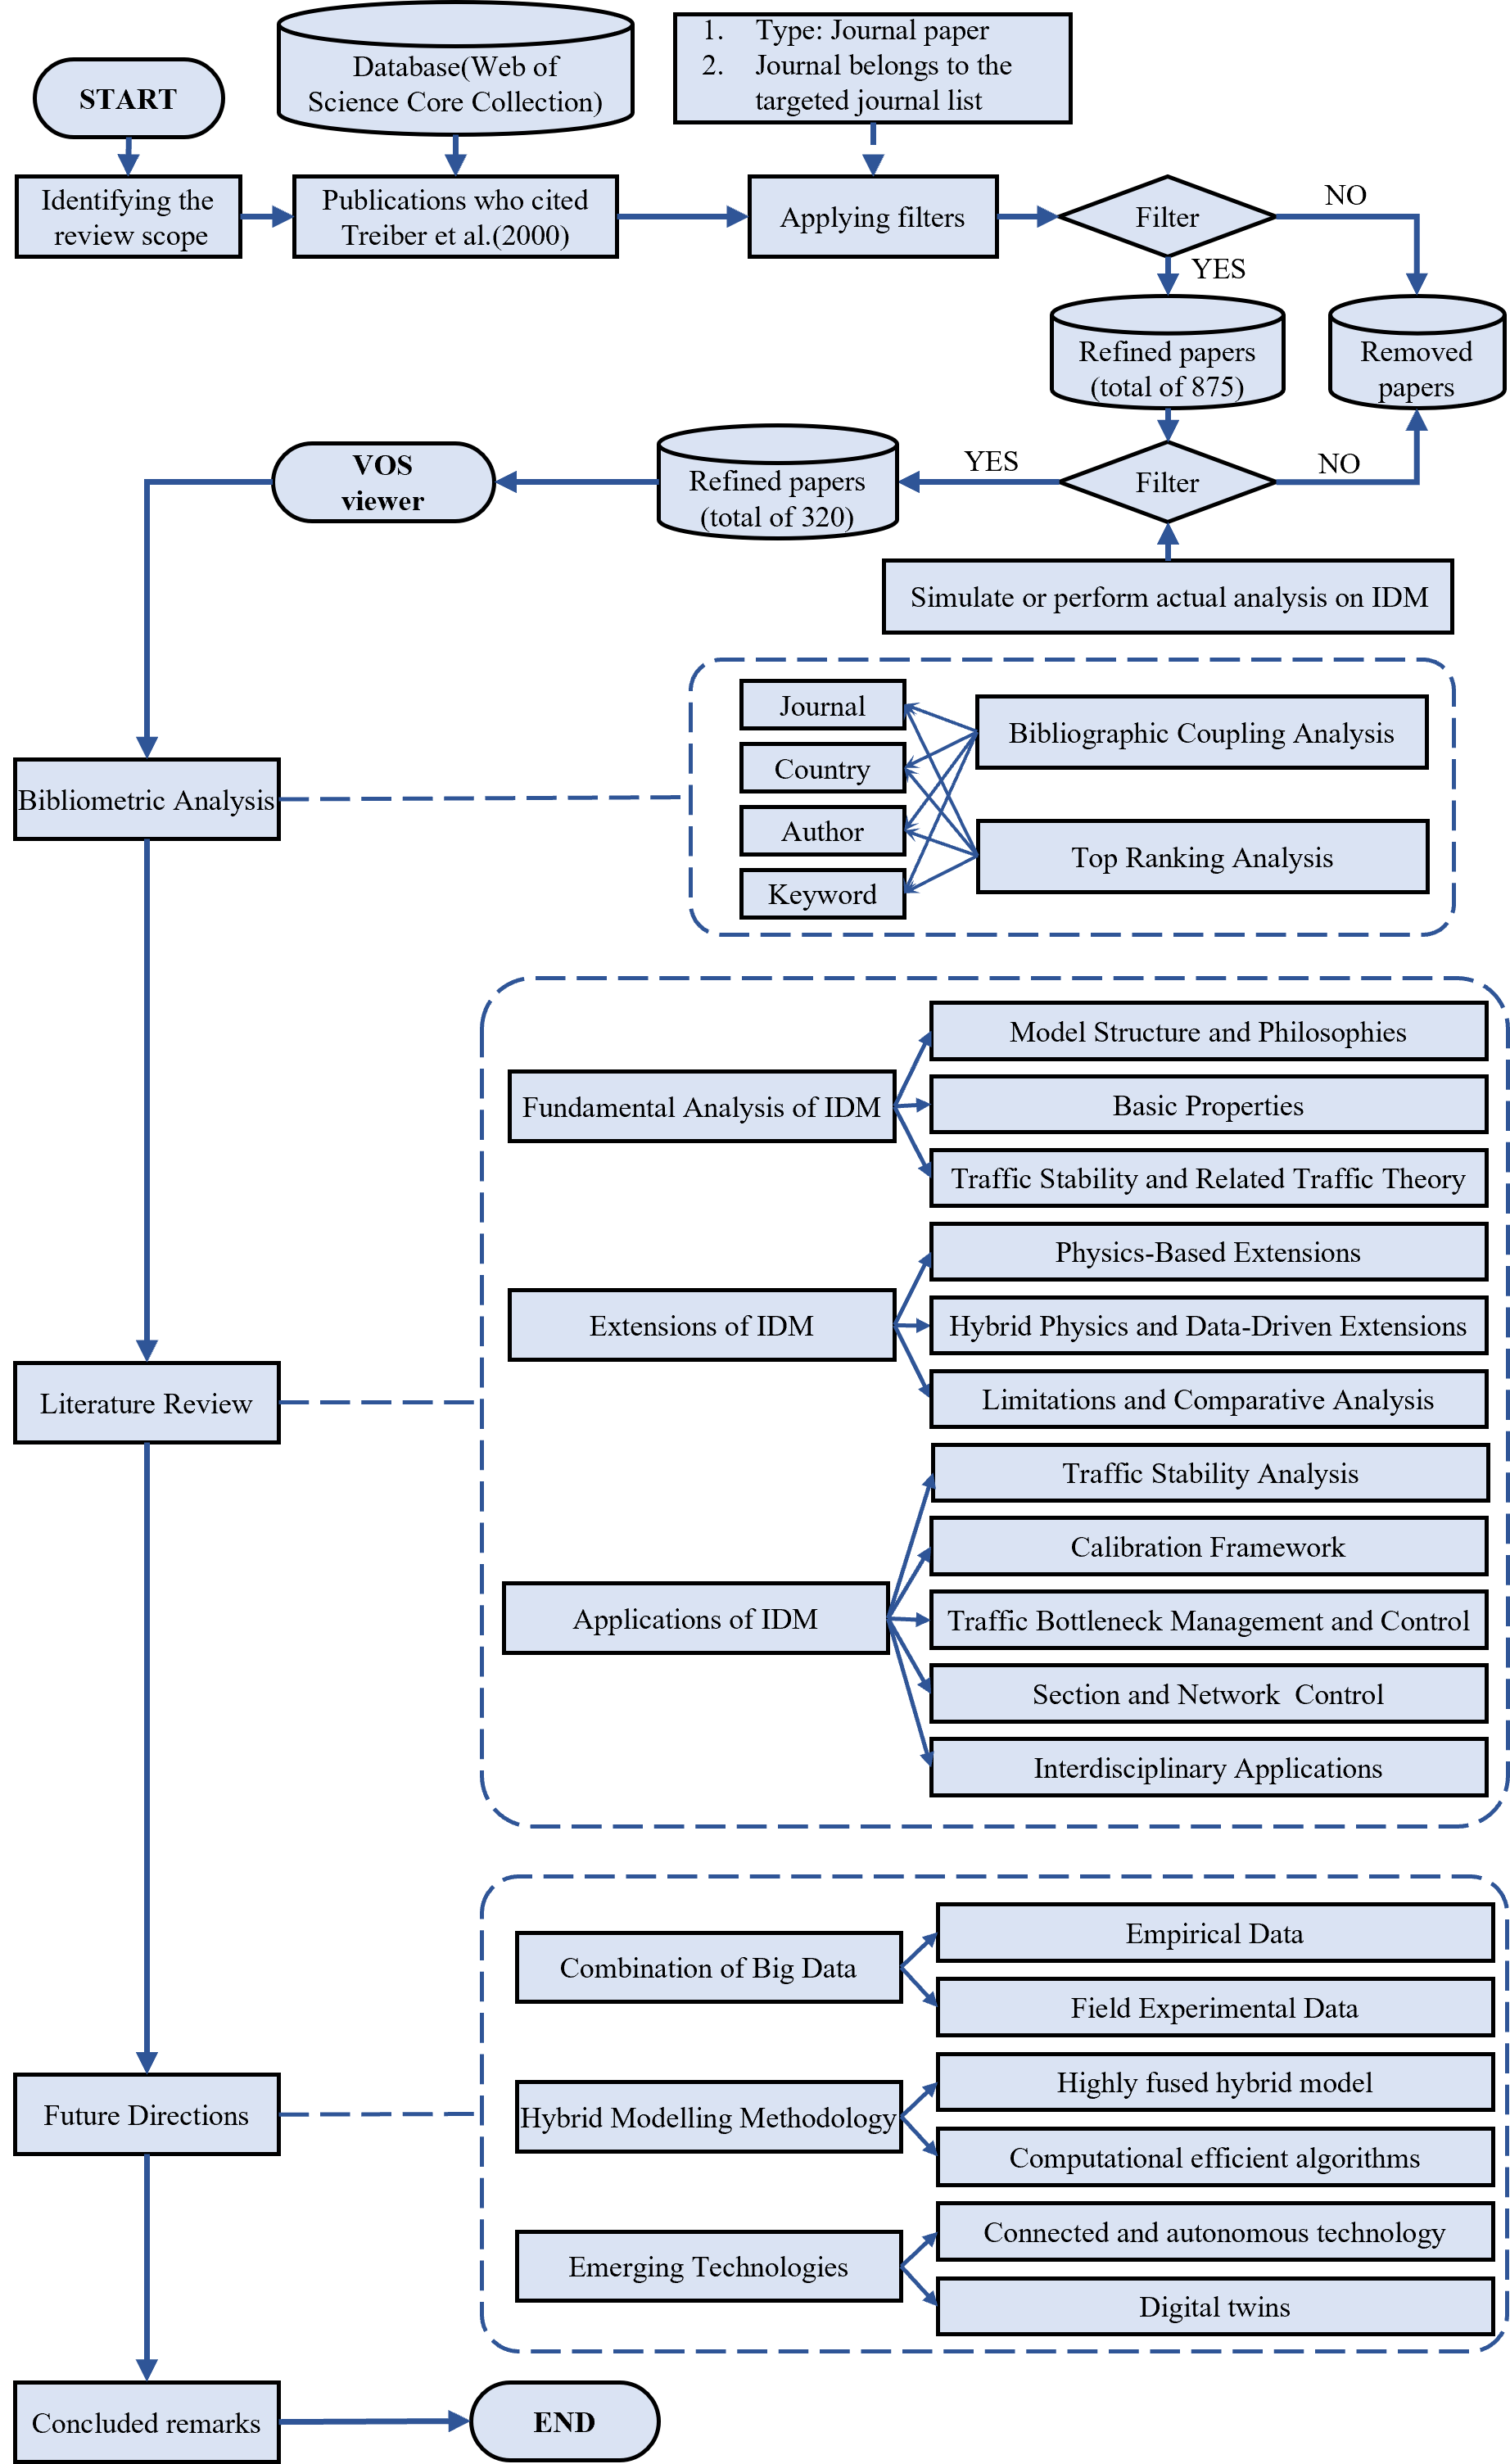
\includegraphics[width=0.85\linewidth]{Figure/Framework.png}
    \caption{Research Framework}
    \label{fig:frm}
\end{figure}

\section{Bibliometric analysis}

This section offers a detailed bibliometric analysis of research on the IDM. By employing quantitative techniques, we classify bibliometric data to generate comprehensive summaries. Bibliometric analysis is a recognized method for assessing the impact of journals, institutions, and researchers, as well as exploring research topic characteristics. Using visualization tools like VOSviewer, we construct and display networks such as co-citation, co-authorship, and keyword co-occurrence. To evaluate the influence of publications, authors, and journals, various metrics are considered, including the number of publications, total citations, and average citations per article.

To build our bibliometric dataset, we utilized the Web of Science Core Collection. Unlike traditional keyword searches, our approach directly focuses on articles citing the seminal IDM work by \cite{treiberCongestedTrafficStatesEmpirical2000}. Given IDM’s high citation count of 2,786 (as of Dec. 2024), we established screening criteria to focus on the most relevant studies. First, we referred to a target journal list based on \cite{punzoCalibrationCarFollowingDynamicsAutomated2021c}. Second,studies citing IDM only in literature reviews without substantial analysis or application were excluded. Both the bibliometric analysis in Section 2 and the literature review in Section 3 are derived from this carefully filtered dataset. Ultimately, this process resulted in a selection of 313 relevant papers, allowing us to provide a precise and exhaustive analysis of IDM's academic impact. Table \ref{tab:CFModel} indicates that since its introduction in 2000, the IDM has garnered 2,786 citations, averaging 111.44 citations per year (CPY). It ranks first in both total citations and CPY among classic car following models. Morever, compared to more general models of traffic flow, although IDM have not acquired highest citations, its CPY is alway rank first, see Table \ref{tab:trafficmodel}.

{
\begin{table}[H]
\centering
\caption{Citations of famous classic car following models included in the Web of Science Core Collection as of Dec. 2024. \cite{wiedemann1992microscopic} is not included in the web of science, so the citation is collected in google scholar database.  }
\scriptsize
\label{tab:CFModel}
\begin{tblr}{
  width = \linewidth,
  colspec = {Q[56]Q[240]Q[306]Q[158]Q[110]Q[69]},
  cells = {c},
  hline{1,12} = {-}{0.08em},
  hline{2} = {-}{},
}
Citations & Classic Models & Title & Publication Source & Citations  Per Year(CPY) & Rank by CPY\\
2786 & {IDM \\\citep{treiberCongestedTrafficStatesEmpirical2000}} & Congested Traffic States in Empirical Observations and Microscopic Simulations & Physical Review E & 111.44 & 1\\
2307 & {Optimal Velocity Model \\\citep{bandoDynamicalModelTrafficCongestion1995a}} & Dynamical model of traffic congestion and numerical simulation & Physical Review E & 76.90 & 2\\
1425 & {Gipps Model \\\citep{gippsBehaviouralCarfollowingModelComputer1981a}} & A behavioural car-following model for computer simulation & Transportation Research Part B & 32.39 & 4\\
1139 & {Full Velocity Difference Model \\\citep{jiangFullVelocityDifferenceModel2001a}} & Full velocity difference model for a car-following theory & Physical Review E & 47.46 & 3\\
957 & {GHR Model \\\citep{gazisNonlinearFollowLeaderModelsTraffic1961}} & Nonlinear follow-the-leader models of traffic flow & Operations Research & 14.95 & 6\\
904 & {General Motor Model \\\citep{chandlerTrafficDynamicsStudiesCar1958}} & Traffic dynamics: studies in car following & Operations Research & 13.49 & 8\\
902 & {Newell Nonlinear Model \\\citep{newellNonlinearEffectsDynamicsCar1961a}} & Nonlinear effects in the dynamics of car following & Operations Research & 14.09 & 7\\
851 & {Pipes Model \\\citep{pipesOperationalAnalysisTrafficDynamics1953}} & An operational analysis of traffic dynamics & Journal of applied physics & 11.82 & 9\\
609 & {Newell Simplified Model \\\citep{newellSimplifiedCarfollowingTheoryLower2002}} & A simplified car-following theory: a lower order model & Transportation Research Part B & 26.48 & 5\\
349 & {Wiedemann Model\\\citep{wiedemann1992microscopic}} & Microscopic traffic simulation: the simulation system MISSION & Project ICARUS (V1052) Final Report & 10.58 & 10
\end{tblr}
\end{table}
}

{
\begin{table}
\centering
\caption{Citations of famous models in transportation research field included in the Web of Science Core Collection as of Dec. 2024. }
\scriptsize
\label{tab:trafficmodel}
\begin{tblr}{
  width = \linewidth,
  colspec = {Q[52]Q[198]Q[363]Q[158]Q[98]Q[62]},
  cells = {c},
  hline{1-2,7} = {-}{},
}
Citations & Classic Models & Title & Publication Source & Citations Per Year(CPY) & Rank by CPY\\
2786 & {IDM \\\cite{treiberCongestedTrafficStatesEmpirical2000}} & Congested traffic states in empirical observations and microscopic  simulations & Physical Review E & 111.44 & 1\\
3382 & {NaSch\\\cite{nagelCellularAutomatonModelFreeway1992a}} & A cellular automaton model for freeway traffic & Journal De Physique & 102.48 & 2\\
2216 & {CTM\\\cite{daganzoCellTransmissionModelDynamic1994}} & The cell  transmission model-a dynamic representation of highway traffic consistent with the hydrodynamic theory & Transportation Research Part B & 71.48 & 3\\
3231 & {LWR \\\cite{lighthillKinematicWavesIITheory1955}} & On kinematic waves  II. a theory of traffic flow on long crowded roads & Proceedings of the Royal Society of London & 46.16 & 4\\
1519 & {Vickrey's bottleneck model\\\cite{vickreyCongestionTheoryTransportInvestment1969}} & Congestion theory and transport investment & American Economic Review & 27.13 & 5
\end{tblr}
\end{table}
}

Fig. \ref{fig:NumPaper} shows the distribution of papers published during 2000-2024 in the target journal and all journals. Blue bars represent publications in the target journal, while red bars represent those in all journals. Initially, from 2001 to 2009, there was minimal activity, with only a few papers published. However, from 2010 onwards, increasing attention led to a noticeable rise in publications. The period 2022-2024 saw a significant peak with 168 papers (53.8\%)  in the target journal and 808(39.3\%) across all journals. This trend indicates the growing importance and popularity of the research topic, which is expected to continue in the future.

Table \ref{tab:TopJou} highlights the top 10 journals (out of 29) that have published more than four papers. Since some journal titles are too long, we defined abbreviations and used them in the rest of the article. These journals primarily fall within the "Transportation," "Economics," "Civil," and "Energy" categories according to the Journal Citation Reports (JCR) by Thomson Reuters. This indicates the broad application and development of IDM across diverse fields. IEEE Transactions on Intelligent Transportation Systems (IEEE-TITS) leads with 114 related papers, followed by Transportation Research Part C (TR-C) with 84 papers, underscoring IDM's significant application value in transportation technology. Notably, Transportation Research Part B (TR-B), renowned for its methodological innovations, features over 20 papers involving IDM research. Importantly, our statistics include papers that have at least applied IDM in simulations, rather than merely citing \cite{treiberCongestedTrafficStatesEmpirical2000}, which would result in a much higher count.

\begin{figure}[htbp]
    \centering
    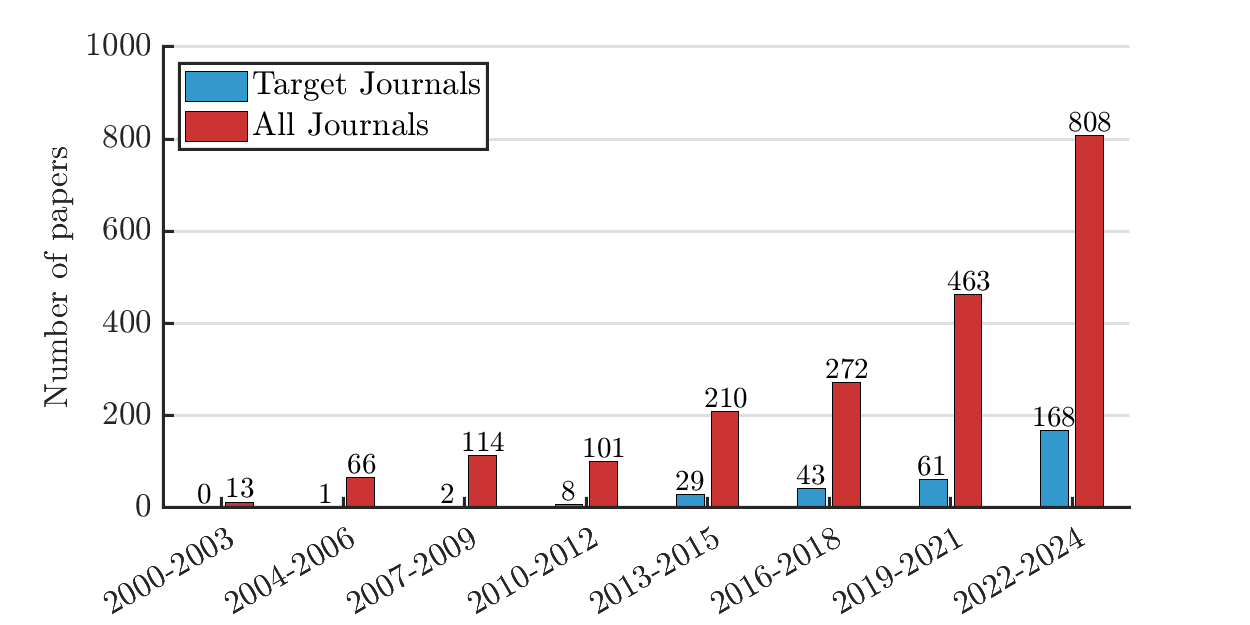
\includegraphics[width=1\linewidth]{Figure/NoP.png}
    \caption{Number of relevant papers published during 2000-2024. Blue and red bars represent the relevant papers published in target journal list and in all journals in the web of science core collection, respectively.}
    \label{fig:NumPaper}
\end{figure}


{
\begin{table}[htbp]
\centering
\caption{Top journals by the number of published related papers.}
\scriptsize
\label{tab:TopJou}
\begin{tblr}{
  width = \linewidth,
  colspec = {Q[58]Q[469]Q[133]Q[281]},
  cells = {c},
  hline{1,14} = {-}{0.08em},
  hline{2} = {-}{},
}
Rank & Journal & Abbreviations & Total number of relevant  papers\\
1 & IEEE Transactions on Intelligent Transportation Systems & IEEE-TITS & 114\\
2 & Transportation Research  Part C & TR-C & 84\\
3 & IEEE Transactions on Vehicular Technology & IEEE-TVT & 25\\
4 & Transportation Research Part B & TR-B & 23\\
5 & Accident Analysis and Prevention & AAP & 14\\
6 & IEEE Transactions on Intelligent Vehicles & IEEE-TIV & 12\\
7 & Physica A & - & 8\\
8 & Computer-Aided Civil and Infrastructure Engineering & CACIE & 6\\
9 & Energy & - & 5\\
9 & Physical Review E & PRE &5\\
11 & Applied Energy & - & 4\\
11 & Transportation Research Part D & TR-D & 4\\
\end{tblr}
\end{table}
}


\begin{figure}[htbp]
    \centering
    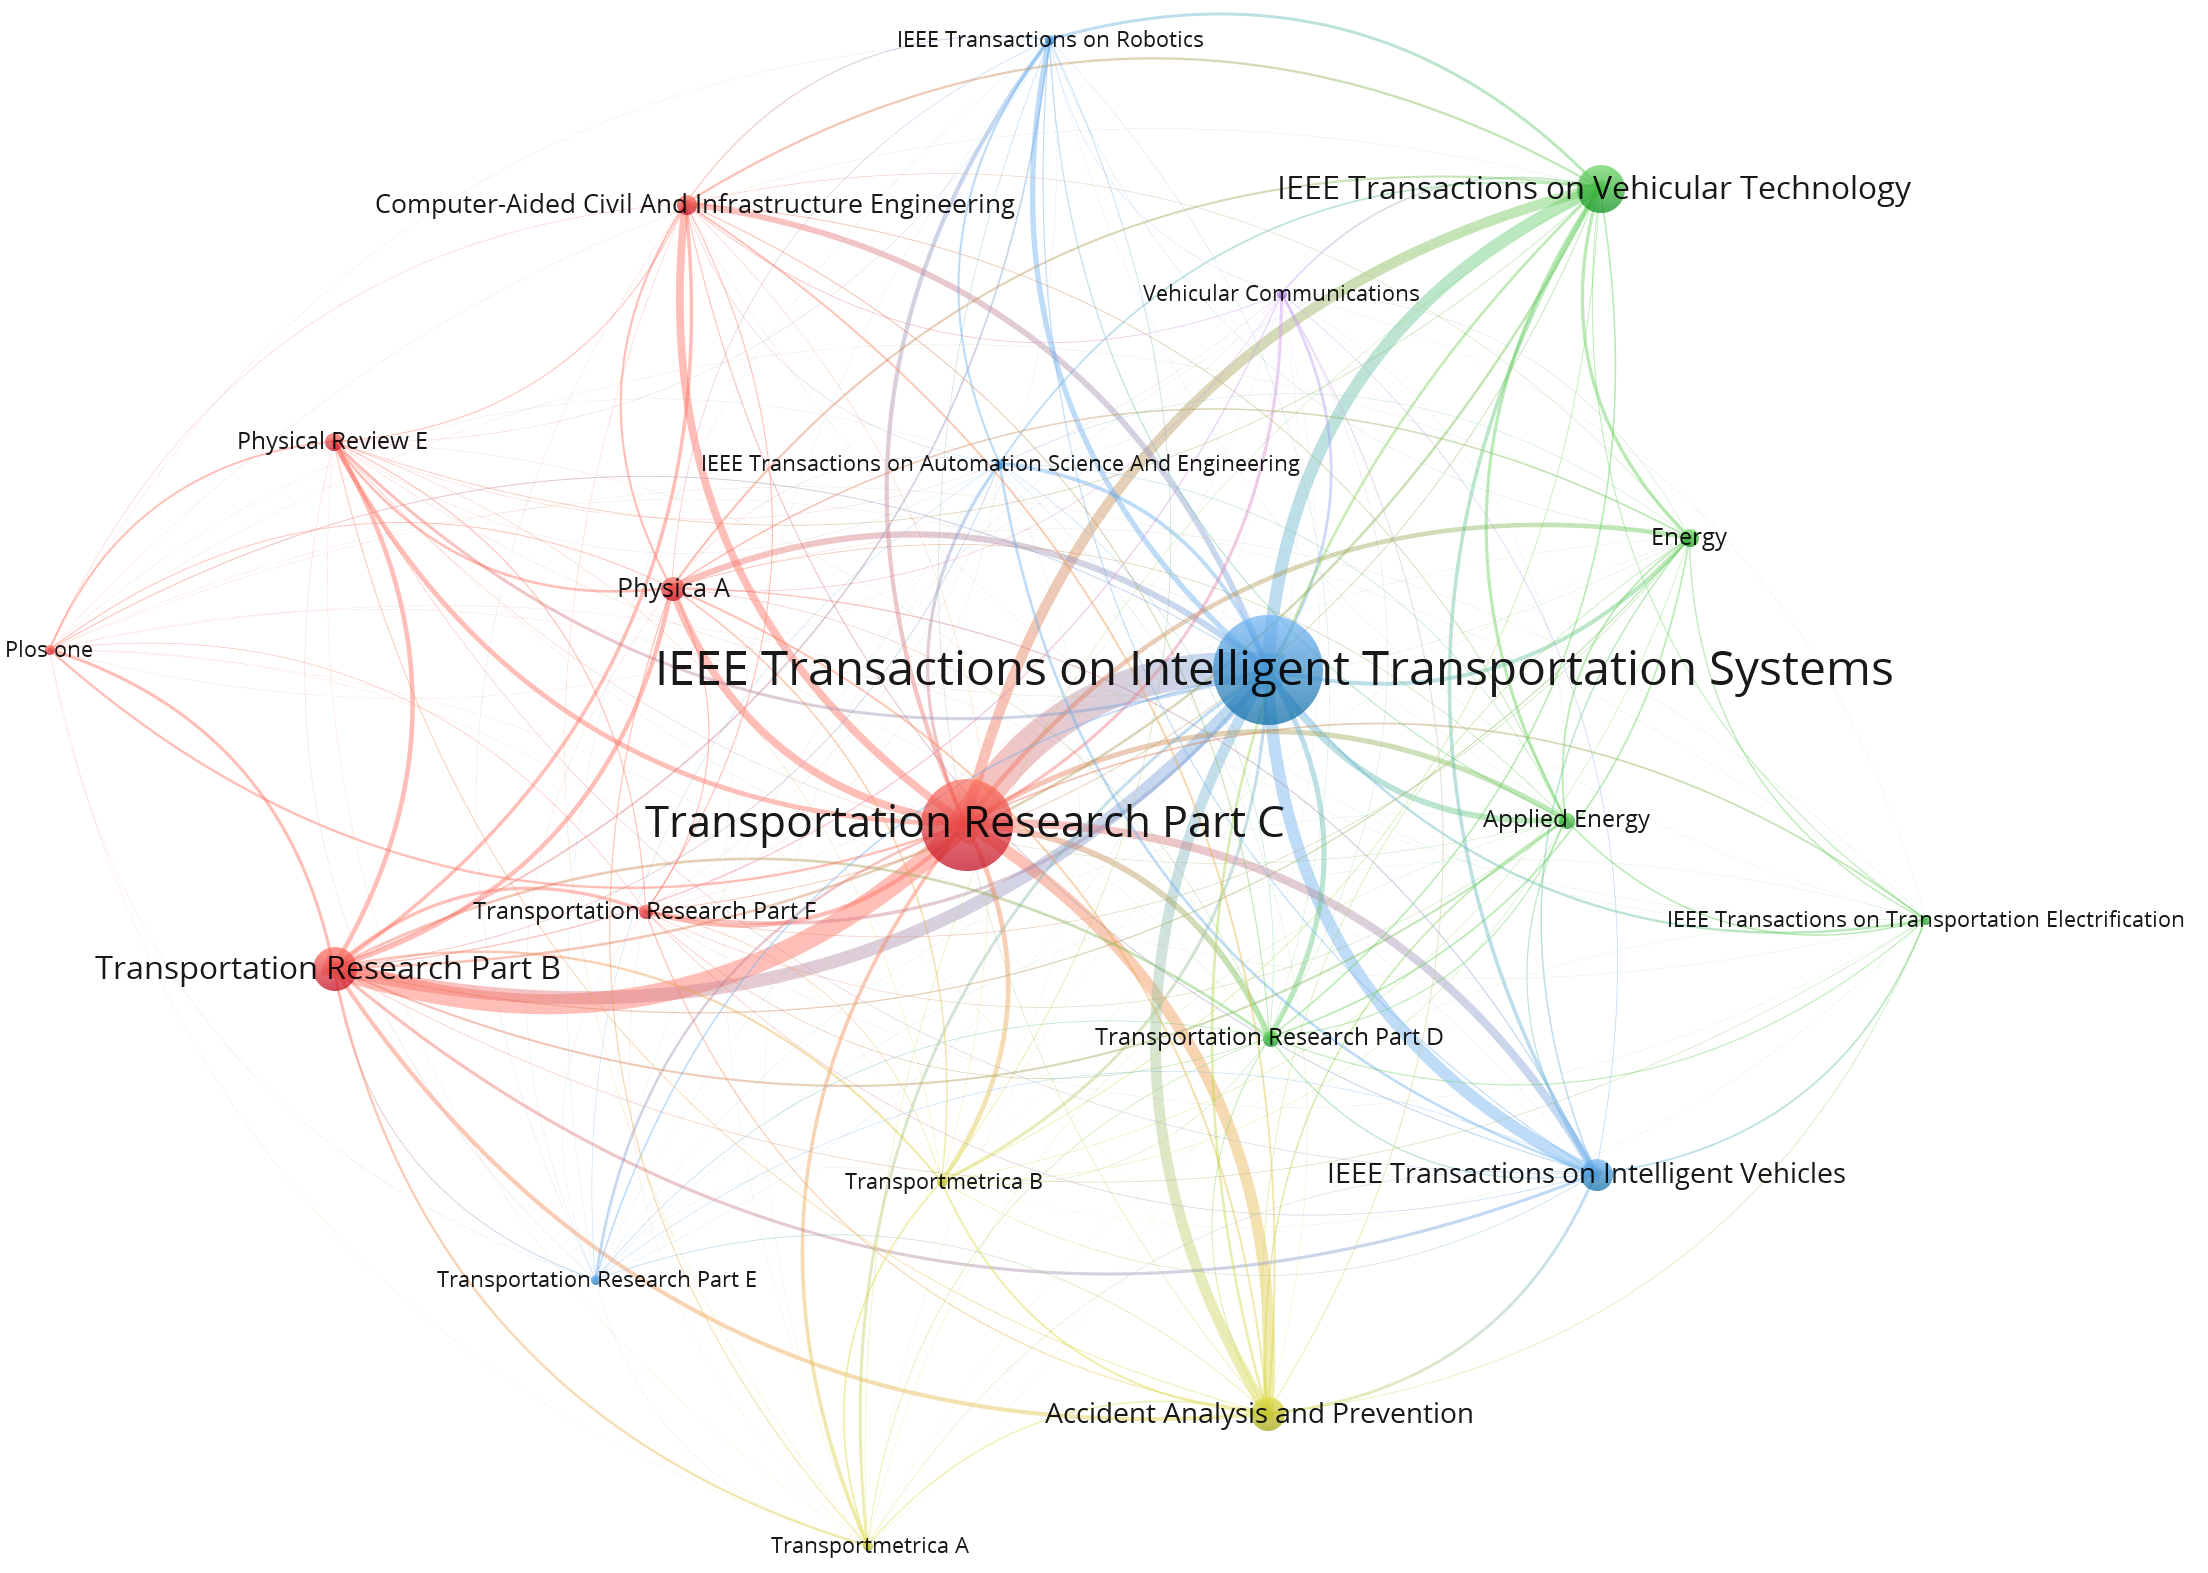
\includegraphics[width=1\linewidth]{Figure/Journal.png}
    \caption{Bibilographic coupling of journals.}
    \label{fig:BibJou}
\end{figure}



To analyze the coupling relationships among journals, we calculated the coupling strength between each pair of journals by normalizing the number of co-citations based on the number of publications in each journal in Fig. \ref{fig:BibJou}. The size of each circle represents the number of publications related to the topic within each journal. The lines between circles indicate the co-citation relationships. The thickness of the lines signifies the degree of co-citation intensity between journals. Specifically, thicker lines indicate a stronger co-citation relationship. It can be observed that papers in TR-C are frequently cited by those in IEEE-TITS, IEEE-TIV, and TR-B. Additionally, IEEE-ITS has strong citation connections with TR-C, AAP, and Applied Energy, highlighting a significant interdisciplinary impact.

Table \ref{fig:TopPap} presents the top 50 most cited papers, each garnering at least 40 citations. Citation counts are based on the Scopus database, with rankings determined by total citations and average annual citations. Leading in total citations are papers by \cite{talebpourInfluenceConnectedAutonomousVehicles2016a}, \cite{milanesModelingCooperativeAutonomousAdaptive2014b}, and \cite{kestingAdaptiveCruiseControlDesign2008}, all published in TR-C. Notably, \cite{talebpourInfluenceConnectedAutonomousVehicles2016a} examined the impact of connected and autonomous vehicles (CAV) on traffic flow stability, achieving the highest total citations at 880 and ranking first in average annual citations with 97.78. During the study period, 38 papers exceeded 200 citations, and 43 papers averaged more than 10 citations per year. Among the top 50 papers by total citations, 20 are from TR-C, 14 from IEEE-TITS, 4 from TR-B, and 3 from AAP and Physica A.

{\scriptsize
\begin{longtblr}[
  label= fig:TopPap,
  caption={The top 50 most cited papers.}
]{ 
  width = \linewidth,
  colspec = {Q[52]Q[173]Q[35]Q[448]Q[75]Q[94]Q[56]},
  cells = {c},
  hline{1,52} = {-}{0.08em},
  hline{2} = {-}{},
}
Rank by TC & document & TC & Title & Authors/ Year & Citations
  Per Year(CPY)~ & Rank by CPY\\
1 & TR-C & 880 & Influence of Connected and Autonomous Vehicles on Traffic Flow Stability
  and Throughput & \cite{talebpourInfluenceConnectedAutonomousVehicles2016a} & 97.78 & 1\\
2 & TR-C & 690 & Modeling Cooperative and Autonomous Adaptive Cruise Control Dynamic
  Responses Using Experimental Data & \cite{milanesModelingCooperativeAutonomousAdaptive2014b} & 62.73 & 2\\
3 & TR-C & 419 & Adaptive Cruise Control Design for Active Congestion Avoidance & \cite{kestingAdaptiveCruiseControlDesign2008} & 24.65 & 16\\
4 & Physica A & 375 & Delays, Inaccuracies and Anticipation in Microscopic Traffic Models & \cite{treiber_delays_2006} & 19.74 & 32\\
5 & TR-C & 307 & Modeling Car-Following Behavior on Urban Expressways in Shanghai: A
  Naturalistic Driving Study & \cite{zhuModelingCarFollowingBehaviorUrban2018b} & 43.86 & 3\\
6 & TR-C & 306 & Incorporating Human-Factors in Car-Following Models: A Review of Recent
  Developments and Research Needs & \cite{saifuzzamanIncorporatingHumanFactorsCarFollowingModels2014c} & 27.82 & 12\\
7 & TR-C & 238 & Eco Approaching at an Isolated Signalized Intersection under Partially
  Connected and Automated Vehicles Environment & \cite{jiangEcoApproachingIsolatedSignalized2017a} & 29.75 & 7\\
8 & IEEE-TITS & 231 & Platooning with IVC-enabled autonomous vehicles: Strategies to mitigate
  communication delays, improve safety and traffic flow & \cite{fernandes_platooning_2012} & 17.77 & 37\\
9 & TR-C & 214 & Rolling Horizon Control Framework for Driver Assistance Systems. Part II:
  Cooperative Sensing and Cooperative Control & \cite{wangRollingHorizonControlFramework2014b} & 19.45 & 33\\
10 & TR-B & 205 & Trajectory Data Reconstruction and Simulation-Based Validation against
  Macroscopic Traffic Patterns & \cite{montaninoTrajectoryDataReconstructionSimulationBased2015b} & 20.50 & 28\\
11 & IEEE-TITS & 203 & Capturing car-following behaviors by deep learning & \cite{wang_capturing_2018} & 29.00 & 8\\
12 & TR-C & 203 & Variable Speed Limit: A Microscopic Analysis in a Connected Vehicle
  Environment & \cite{khondakerVariableSpeedLimitMicroscopic2015a} & 20.30 & 29\\
13 & AAP & 202 & Longitudinal Safety Evaluation of Connected Vehicles' Platooning on
  Expressways & \cite{rahman_longitudinal_2018} & 28.86 & 9\\
14 & TR-C & 200 & A Recurrent Neural Network Based Microscopic Car Following Model to
  Predict Traffic Oscillation & \cite{zhouRecurrentNeuralNetworkBased2017b} & 25.00 & 15\\
15 & IEEE-TITS & 196 & On the impact of cooperative autonomous vehicles in improving
  freeway merging: a modified intelligent driver model-based approach & \cite{zhou_impact_2017} & 24.50 & 17\\
16 & TR-C & 194 & Isolated Intersection Control for Various Levels of Vehicle Technology:
  Conventional, Connected, and Automated Vehicles & \cite{yangIsolatedIntersectionControlVarious2016a} & 21.56 & 26\\
17 & IEEE-TITS & 181 & Development of an Efficient Driving Strategy for Connected and Automated
  Vehicles at Signalized Intersections: A Reinforcement Learning Approach & \cite{zhou_development_2020} & 36.20 & 4\\
18 & IEEE-TITS & 181 & Optimal control of connected vehicle systems with communication delay and
  driver reaction time & \cite{ge_optimal_2017} & 22.63 & 21\\
19 & IEEE-TITS & 173 & Analysis of recurrent neural networks for probabilistic modeling of
  driver behavior & \cite{morton_analysis_2017} & 21.63 & 25\\
20 & TR-C & 171 & Human-like Autonomous Car-Following Model with Deep Reinforcement
  Learning & \cite{zhuHumanlikeAutonomousCarFollowingModel2018b} & 24.43 & 18\\
21 & TR-C & 166 & Joint Optimization of Vehicle Trajectories and Intersection Controllers
  with Connected Automated Vehicles: Combined Dynamic Programming and Shooting
  Heuristic Approach & \cite{guoJointOptimizationVehicleTrajectories2019a} & 27.67 & 13\\
22 & Applied Energy & 163 & Jointly Dampening Traffic Oscillations and Improving Energy Consumption
  with Electric, Connected and Automated Vehicles: A Reinforcement Learning
  Based Approach & \cite{qu_jointly_2020} & 32.60 & 5\\
23 & TR-B & 162 & On Some Experimental Features of Car-Following Behavior and How to Model
  Them & \cite{jiangExperimentalFeaturesCarFollowingBehavior2015b} & 16.20 & 38\\
24 & AAP & 161 & Evaluation of the Impacts of Cooperative Adaptive Cruise Control on
  Reducing Rear-End Collision Risks on Freeways & \cite{li_evaluating_2017} & 20.13 & 31\\
25 & TR-C & 155 & Unravelling Effects of Cooperative Adaptive Cruise Control Deactivation
  on Traffic Flow Characteristics at Merging Bottlenecks & \cite{xiaoUnravellingEffectsCooperativeAdaptive2018a} & 22.14 & 24\\
26 & TR-C & 153 & Heterogeneity in Car-Following Behavior: Theory and Empirics & \cite{ossenHeterogeneityCarFollowingBehaviorTheory2011b} & 10.93 & 41\\
27 & Plos One & 152 & Traffic experiment reveals the nature of car-following & \cite{jiangTrafficExperimentRevealsNature2014a} & 13.82 & 39\\
28 & AAP & 151 & Evaluating the Safety Impact of Adaptive Cruise Control in Traffic
  Oscillations on Freeways & \cite{li_evaluating_2017} & 18.88 & 34\\
29 & IEEE-TIV & 150 & Combining Planning and Deep Reinforcement Learning in Tactical Decision
  Making for Autonomous Driving & \cite{hoel_combining_2020} & 30.00 & 6\\
30 & TR-B & 149 & Three-Phase Traffic Theory and Two-Phase Models with a Fundamental
  Diagram in the Light of Empirical Stylized Facts & \cite{treiberThreephaseTrafficTheoryTwophase2010} & 9.93 & 42\\
31 & IEEE-TITS & 145 & Heterogeneous traffic mixing regular and connected vehicles: Modeling and
  stabilization & \cite{xie_heterogeneous_2019} & 24.17 & 19\\
32 & CACIE & 142 & How Reaction Time, Update Time, and Adaptation Time Influence the
  Stability of Traffic Flow & \cite{kesting_how_2008} & 8.35 & 47\\
33 & IEEE-TITS & 139 & A decentralized approach for anticipatory vehicle routing using delegate
  multiagent systems & \cite{claes_decentralized_2011} & 9.93 & 43\\
34 & PRE & 122 & Understanding widely scattered traffic flows, the capacity drop, and
  platoons as effects of variance-driven time gaps & \cite{treiberUnderstandingWidelyScatteredTraffic2006} & 6.42 & 48\\
35 & TR-C & 121 & Simultaneous Modeling of Car-Following and Lane-Changing Behaviors Using
  Deep Learning & \cite{zhangSimultaneousModelingCarFollowingLaneChanging2019c} & 20.17 & 30\\
36 & TR-C & 116 & Integrated Macroscopic Traffic Flow, Emission, and Fuel Consumption Model
  for Control Purposes & \cite{zegeyeIntegratedMacroscopicTrafficFlow2013b} & 9.67 & 44\\
37 & TR-C & 115 & A Survey on Autonomous Vehicle Control in the Era of Mixed-Autonomy: From
  Physics-Based to AI-guided Driving Policy Learning & \cite{di_survey_2021} & 28.75 & 10\\
38 & Physica A & 115 & Linear Stability Analysis of Heterogeneous Traffic Flow Considering
  Degradations of Connected Automated Vehicles and Reaction Time & \cite{yao_linear_2021} & 28.75 & 11\\
39 & PRE & 113 & Memory effects in microscopic traffic models and wide scattering in
  flow-density data & \cite{treiberMemoryEffectsMicroscopicTraffic2003} & 5.14 & 50\\
40 & IEEE-TITS & 113 & Cooperative Eco-Driving at Signalized Intersections in a Partially
  Connected and Automated Vehicle Environment & \cite{wang_cooperative_2020} & 22.60 & 22\\
41 & TR-D & 95 & Eco-Driving-Based Cooperative Adaptive Cruise Control of Connected
  Vehicles Platoon at Signalized Intersections & \cite{maEcoDrivingBasedCooperativeAdaptiveCruise2021a} & 23.75 & 20\\
42 & IEEE-TITS & 92 & Do we really need to calibrate all the parameters? Variance-based
  sensitivity analysis to simplify microscopic traffic flow models & \cite{punzo_we_2015} & 9.20 & 45\\
43 & TR-C & 90 & Modeling and Analyzing Cyberattack Effects on Connected Automated
  Vehicular Platoons & \cite{wang_modeling_2020} & 18.00 & 35\\
44 & TR-C & 89 & Analytical Analysis of the Effect of Maximum Platoon Size of Connected
  and Automated Vehicles & \cite{zhou_analytical_2021} & 22.25 & 23\\
45 & IEEE-TITS & 89 & Cooperative Lane Changing Strategies to Improve Traffic Operation and
  Safety Nearby Freeway Off-Ramps in a Connected and Automated Vehicles
  Environment & \cite{zheng_cooperative_2020} & 17.80 & 36\\
46 & TR-B & 87 & Revisiting the Task-Capability Interface Model for
  Incorporating Human Factors into Car-Following Models & \cite{saifuzzamanRevisitingTaskCapabilityInterfaceModel2015a} & 8.70 & 46\\
47 & Energy & 85 & Fuel Consumption and Transportation
  Emissions Evaluation of Mixed Traffic Flow with Connected Automated Vehicles
  and Human-Driven Vehicles on Expressway & \cite{yao_fuel_2021} & 21.25 & 27\\
48 & IEEE-TITS & 85 & Cooperative intersection control based on virtual platooning & \cite{medina_cooperative_2018} & 12.14 & 40\\
49 & IEEE-TITS & 83 & On the impact of virtual traffic lights on carbon emissions mitigation & \cite{ferreira_impact_2012} & 6.38 & 49\\
50 & IEEE-TITS & 81 & Driving Behavior Modeling Using Naturalistic Human Driving Data with
  Inverse Reinforcement Learning & \cite{huang_driving_2022} & 27.00 & 14
\end{longtblr}}


{\begin{table}[htbp]
\centering
\caption{Top eight countries by the number of relevant papers.}
\scriptsize
\label{tab:TopCou}
\begin{tblr}{
  cells = {c},
  hline{1-2,11} = {-}{},
}
Rank & Country & Total number of relevant  papers \\
1 & China (including mainland China, Hong Kong and Taiwan) & 159\\
2 & USA & 110\\
3 & Australia & 28\\
4 & Germany & 23\\
5 & England & 17\\
5 & Netherlands & 17\\
6 & Italy & 16\\
7 & Sweden & 11\\
8 & Canada & 10
\end{tblr}
\end{table}}

\begin{figure}[htbp]
    \centering
    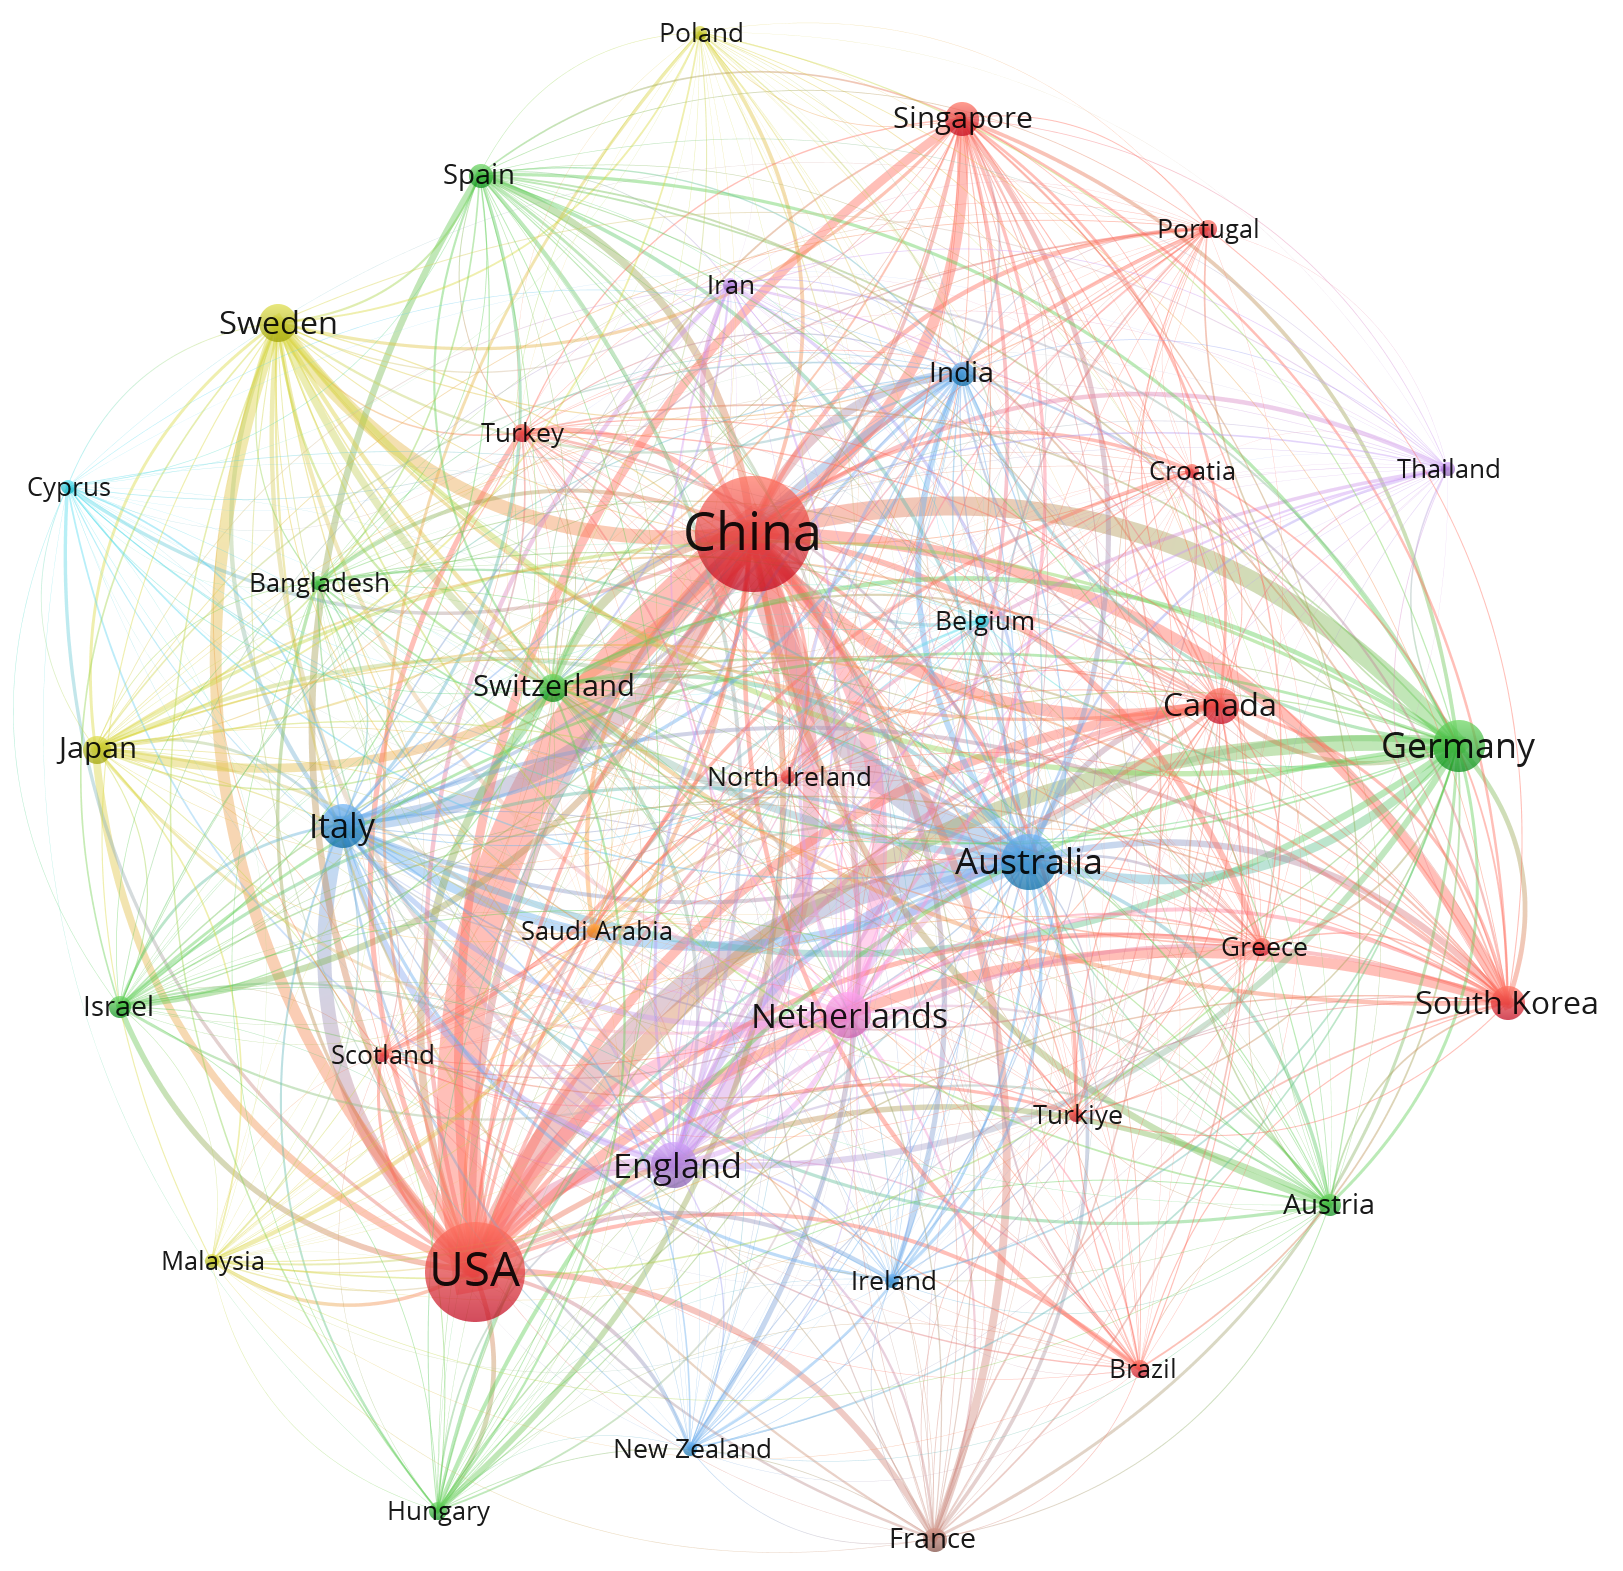
\includegraphics[width=1\linewidth]{Figure/Country.png}
    \caption{Bibilographic coupling of countries.}
    \label{fig:BibCou}
\end{figure}

Figure \ref{fig:BibCou} depicts the collaboration network among 37 countries. Each solid circle represents a country, with its size indicating the number of papers published. The connecting lines represent co-citations, with thickness reflecting the strength of these relationships. Table \ref{tab:TopCou} lists the eight countries that published more than 10 papers. China accounts for nearly half of the total publications (159 out of 313), with the United States also contributing over 100 papers. These two countries significantly exceed others in output. Papers from China and the United States are frequently cited by authors from Germany, Australia, Italy, the Netherlands, and England.


\begin{figure}[htbp]
    \centering
    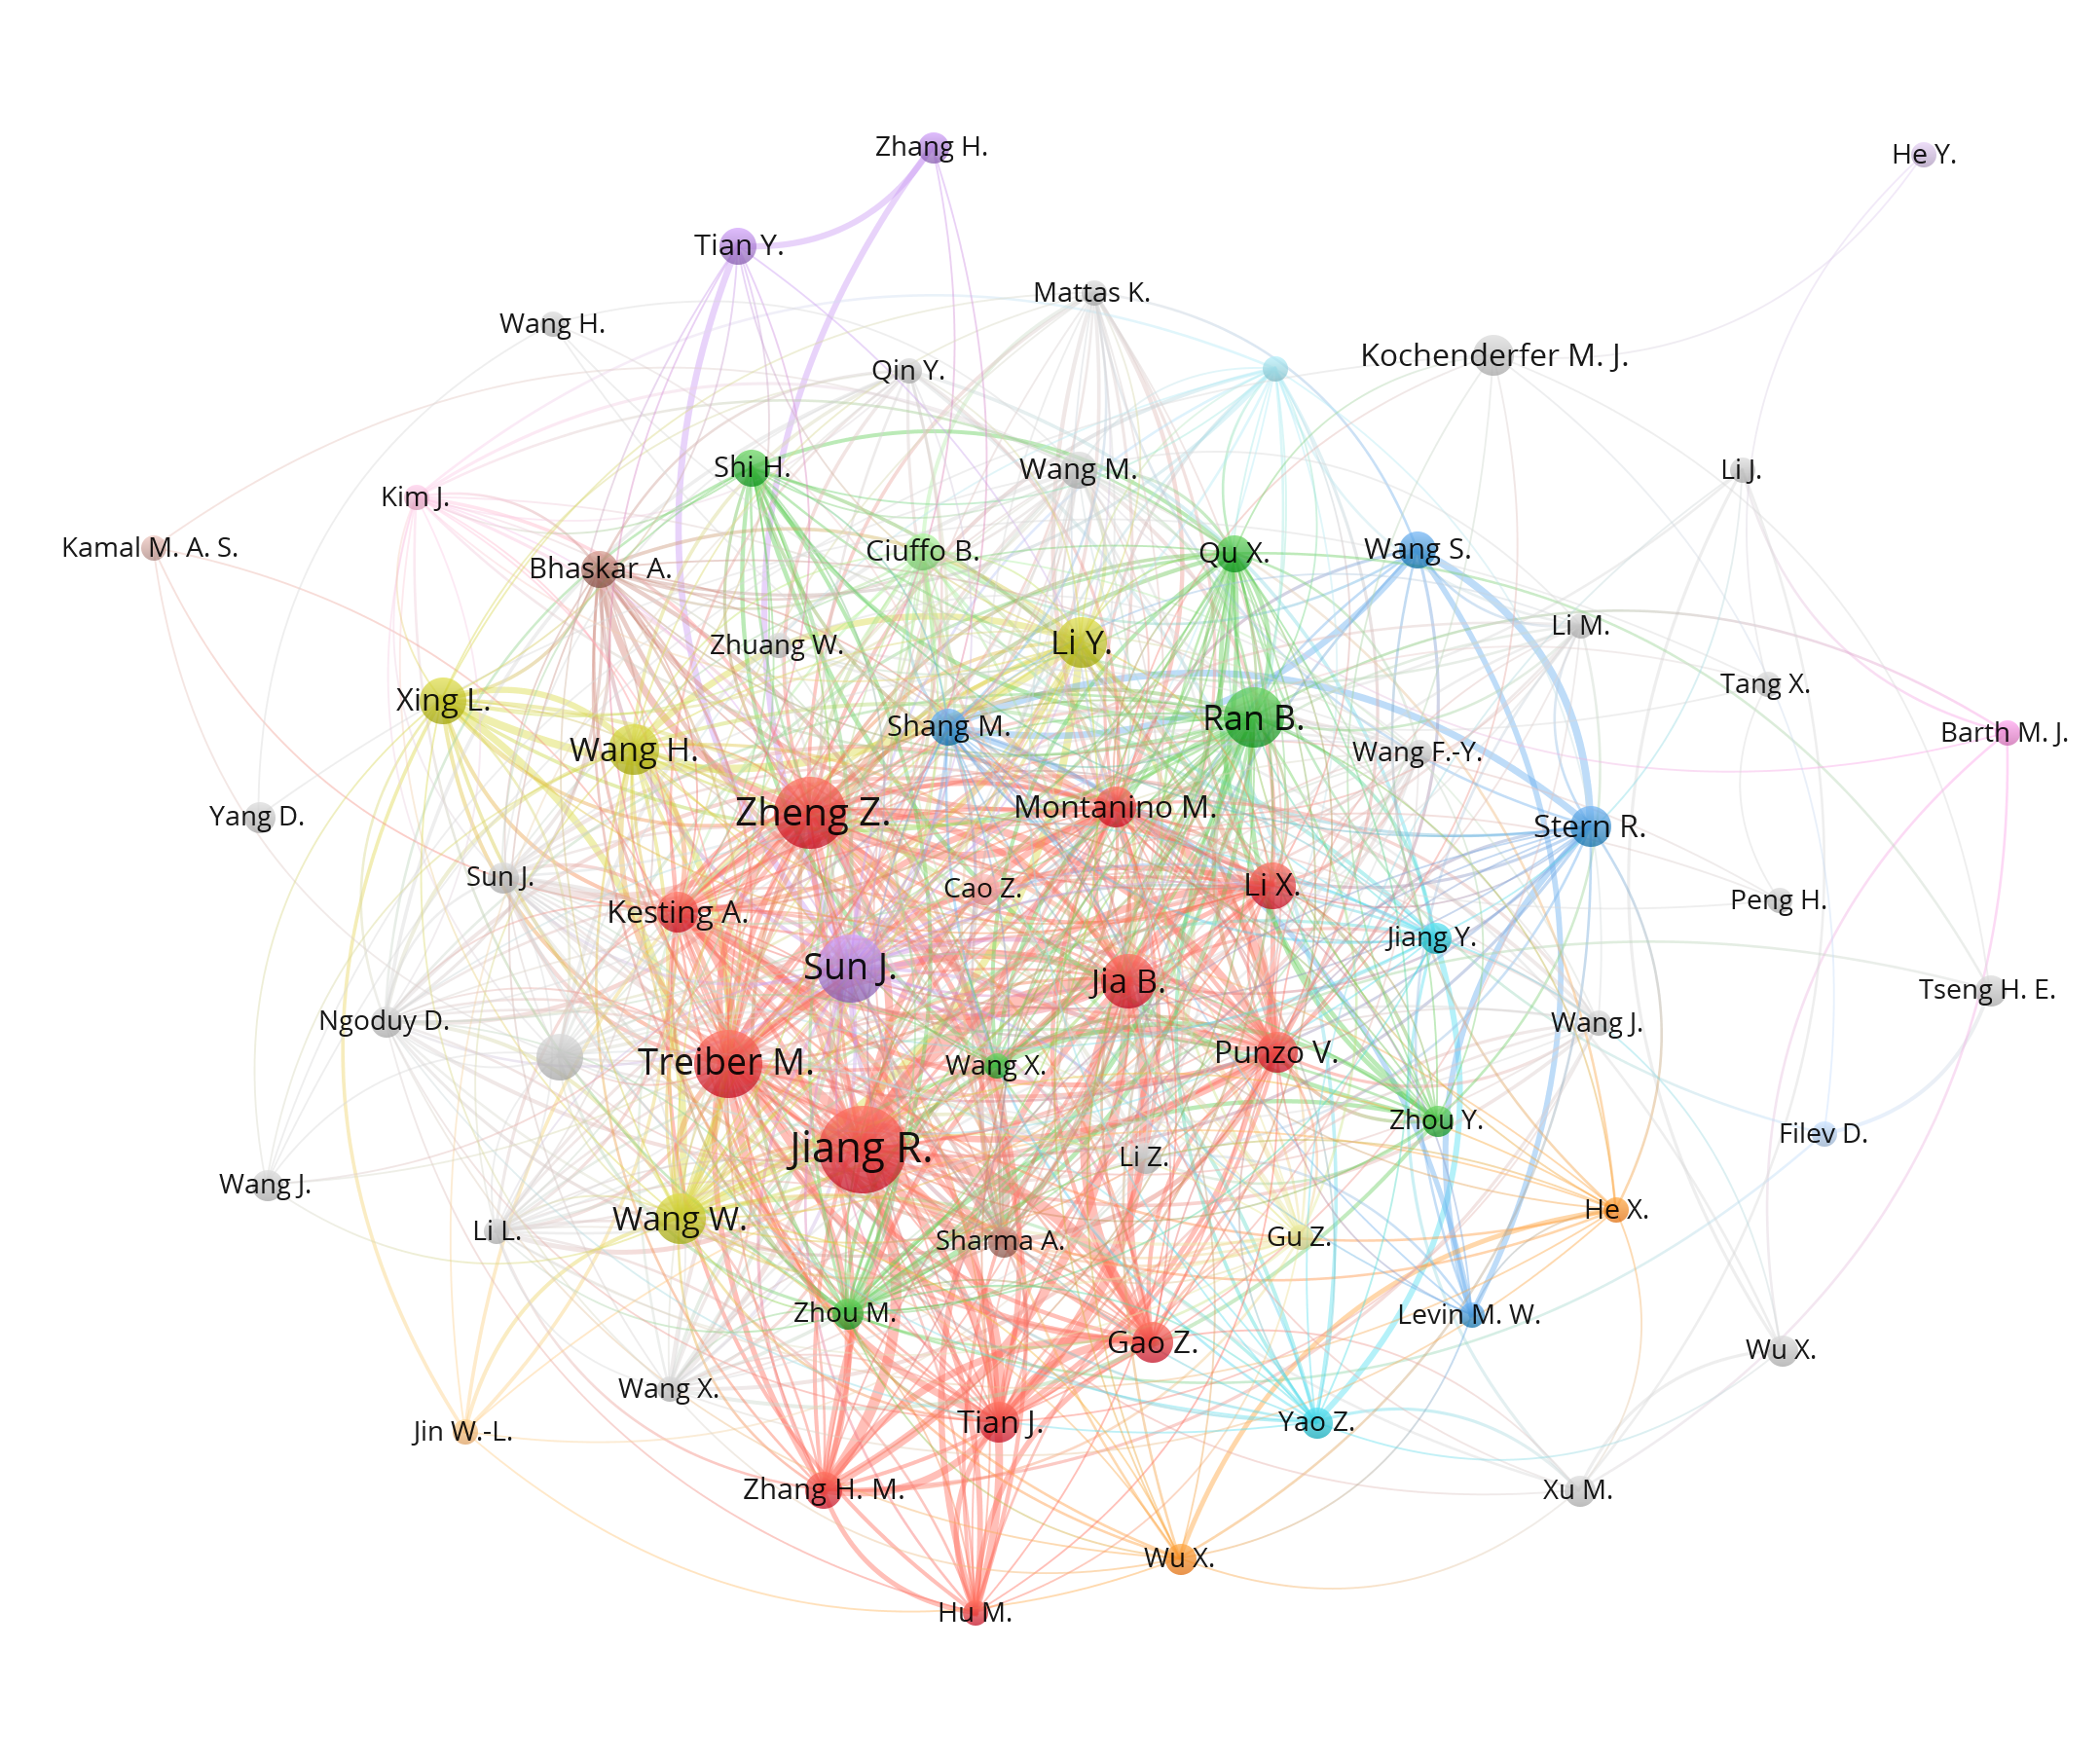
\includegraphics[width=1\linewidth]{Figure/Author.png}
    \caption{Bibilographic coupling of authors.}
    \label{fig:BibAu}
\end{figure}

{
\begin{table}[htbp]
\centering
\caption{Top 28 leading authors with number of papers $\geq$ 5. TP and TC represent the total number of publications and citations, respectively.}
\scriptsize
\begin{tblr}{
  width = \linewidth,
  colspec = {Q[100]Q[156]Q[385]Q[37]Q[54]Q[73]Q[129]},
  cells = {c},
  hline{1,30} = {-}{0.08em},
  hline{2} = {-}{},
}
Rank by TP & Author & Institute and country & TP & TC & TC/TP & Rank by TC/TP\\
1 & Jiang R. & Beijing Jiaotong University, China & 17 & 882 & 51.88 & 19\\
2 &Treiber M. & Dresden University of Technology,
  Germany & 14 & 1277 & 91.21 & 4  \\
3 &  Zheng Z. & University of Queensland, Australia & 13 & 832 & 64.00 & 14\\
4 & Sun J. & Tongji University, China & 12 & 302 & 25.17 & 24\\
5 & Ran B. & University of Wisconsin Madison, USA & 10 & 302 & 30.20 & 22\\
6 & Jia B. & Beijing Jiaotong University, China & 9 & 597 & 66.33 & 12\\
7 & Wang H. & Southeast University, China & 8 & 562 & 70.25 & 9\\
8 & Wang W. & Southeast University, China & 8 & 553 & 69.13 & 11\\
9 & Li Y. & Central South University, China & 8 & 472 & 59.00 & 16\\
10 & Van arem B. & Delft University of Technology,
  Netherlands & 7 & 485 & 69.29 & 10\\
11 & Xing L. & Southeast University, China & 7 & 449 & 64.14 & 13\\
12 & Li X. & University of Wisconsin Madison, USA & 7 & 403 & 57.57 & 17\\
13 & Kesting A. & Dresden University of Technology,
  Germany & 6 & 889 & 148.17 & 2\\
14 & Montanino M. & University of Naples Federico II,
  Italy & 6 & 513 & 85.50 & 6\\
15 & Punzo V. & University
  of Naples Federico II, Italy & 6 & 513 & 85.50 & 7\\
16 & Gao Z. & Beijing Jiaotong University, China & 6 & 506 & 84.33 & 8\\
17 & Kochenderfer M.J. & Stanford University, USA & 6 & 381 & 63.50 & 15\\
18 & Tian J. & Tianjin University, China & 6 & 258 & 43.00 & 21\\
19 & Stern R. & University of Minnesota, USA & 6 & 90 & 15.00 & 26\\
20 & Qu X. & Tsinghua University, China & 5 & 741 & 148.20 & 1\\
21 & Wang M. & Delft University of Technology,
  Netherlands & 5 & 646 & 129.20 & 3\\
22 & Zhang H.M. & University of California Davis, USA & 5 & 440 & 88.00 & 5\\
23 & Bhaskar A. & Queensland University of Technology,
  Australia & 5 & 279 & 55.80 & 18\\
24 & Ciuffo B. & European Commission Joint Research
  Centre, Italy & 5 & 229 & 45.80 & 20\\
25 & Shi H. & University of Wisconsin Madison, USA & 5 & 139 & 27.80 & 23\\
26 & Shang M. & University of Minnesota, USA & 5 & 114 & 22.80 & 25\\
27 & Tian Y. & Tongji University, China & 5 & 63 & 12.60 & 27\\
28 & Wang S. & University of Minnesota, USA & 5 & 61 & 12.20 & 28
\end{tblr}
\label{tab:TopAu}
\end{table}
}

Figure \ref{fig:BibAu} shows the bibliographic coupling network of authors, which can help understand the co-citation relationship between authors in IDM-related research fields. The solid circle represents an author, and its size represents the number of papers published by the author. The lines between authors represent the co-citations of authors, and the thickness of the lines represents the corresponding co-citation strength. As many as 856 authors appear in these papers. The network was built using the full count method, with the minimum number of authors set to 3, and the number of authors that met the threshold was 70. In terms of the total number of relevant publications, authors such as Jiang R., Treiber M. , Zheng Z. and Sun J.  are the most influential because they are associated with the big circle. Table \ref{tab:TopAu} highlights the top 28 leading authors, each with at least five publications, detailing their total number of publications, citations, and average citations per paper. The table also specifies the authors' affiliated institutions and countries. Jiang R. tops the list with 17 publications, followed by Zheng Z. and Treiber M. with 13 and 12 publications respectively. Nine authors have published more than eight papers. Kesting A., Van Arem B., and Qu X. are among the top five most influential authors in terms of average citations per paper. Treiber M. leads in total citations with 1118, while Qu X. has the highest average citations per paper at 148.20. Another notable author with a high citation average is Kesting A., with 148.17 citations per paper.


\begin{figure}[htbp]
    \centering
    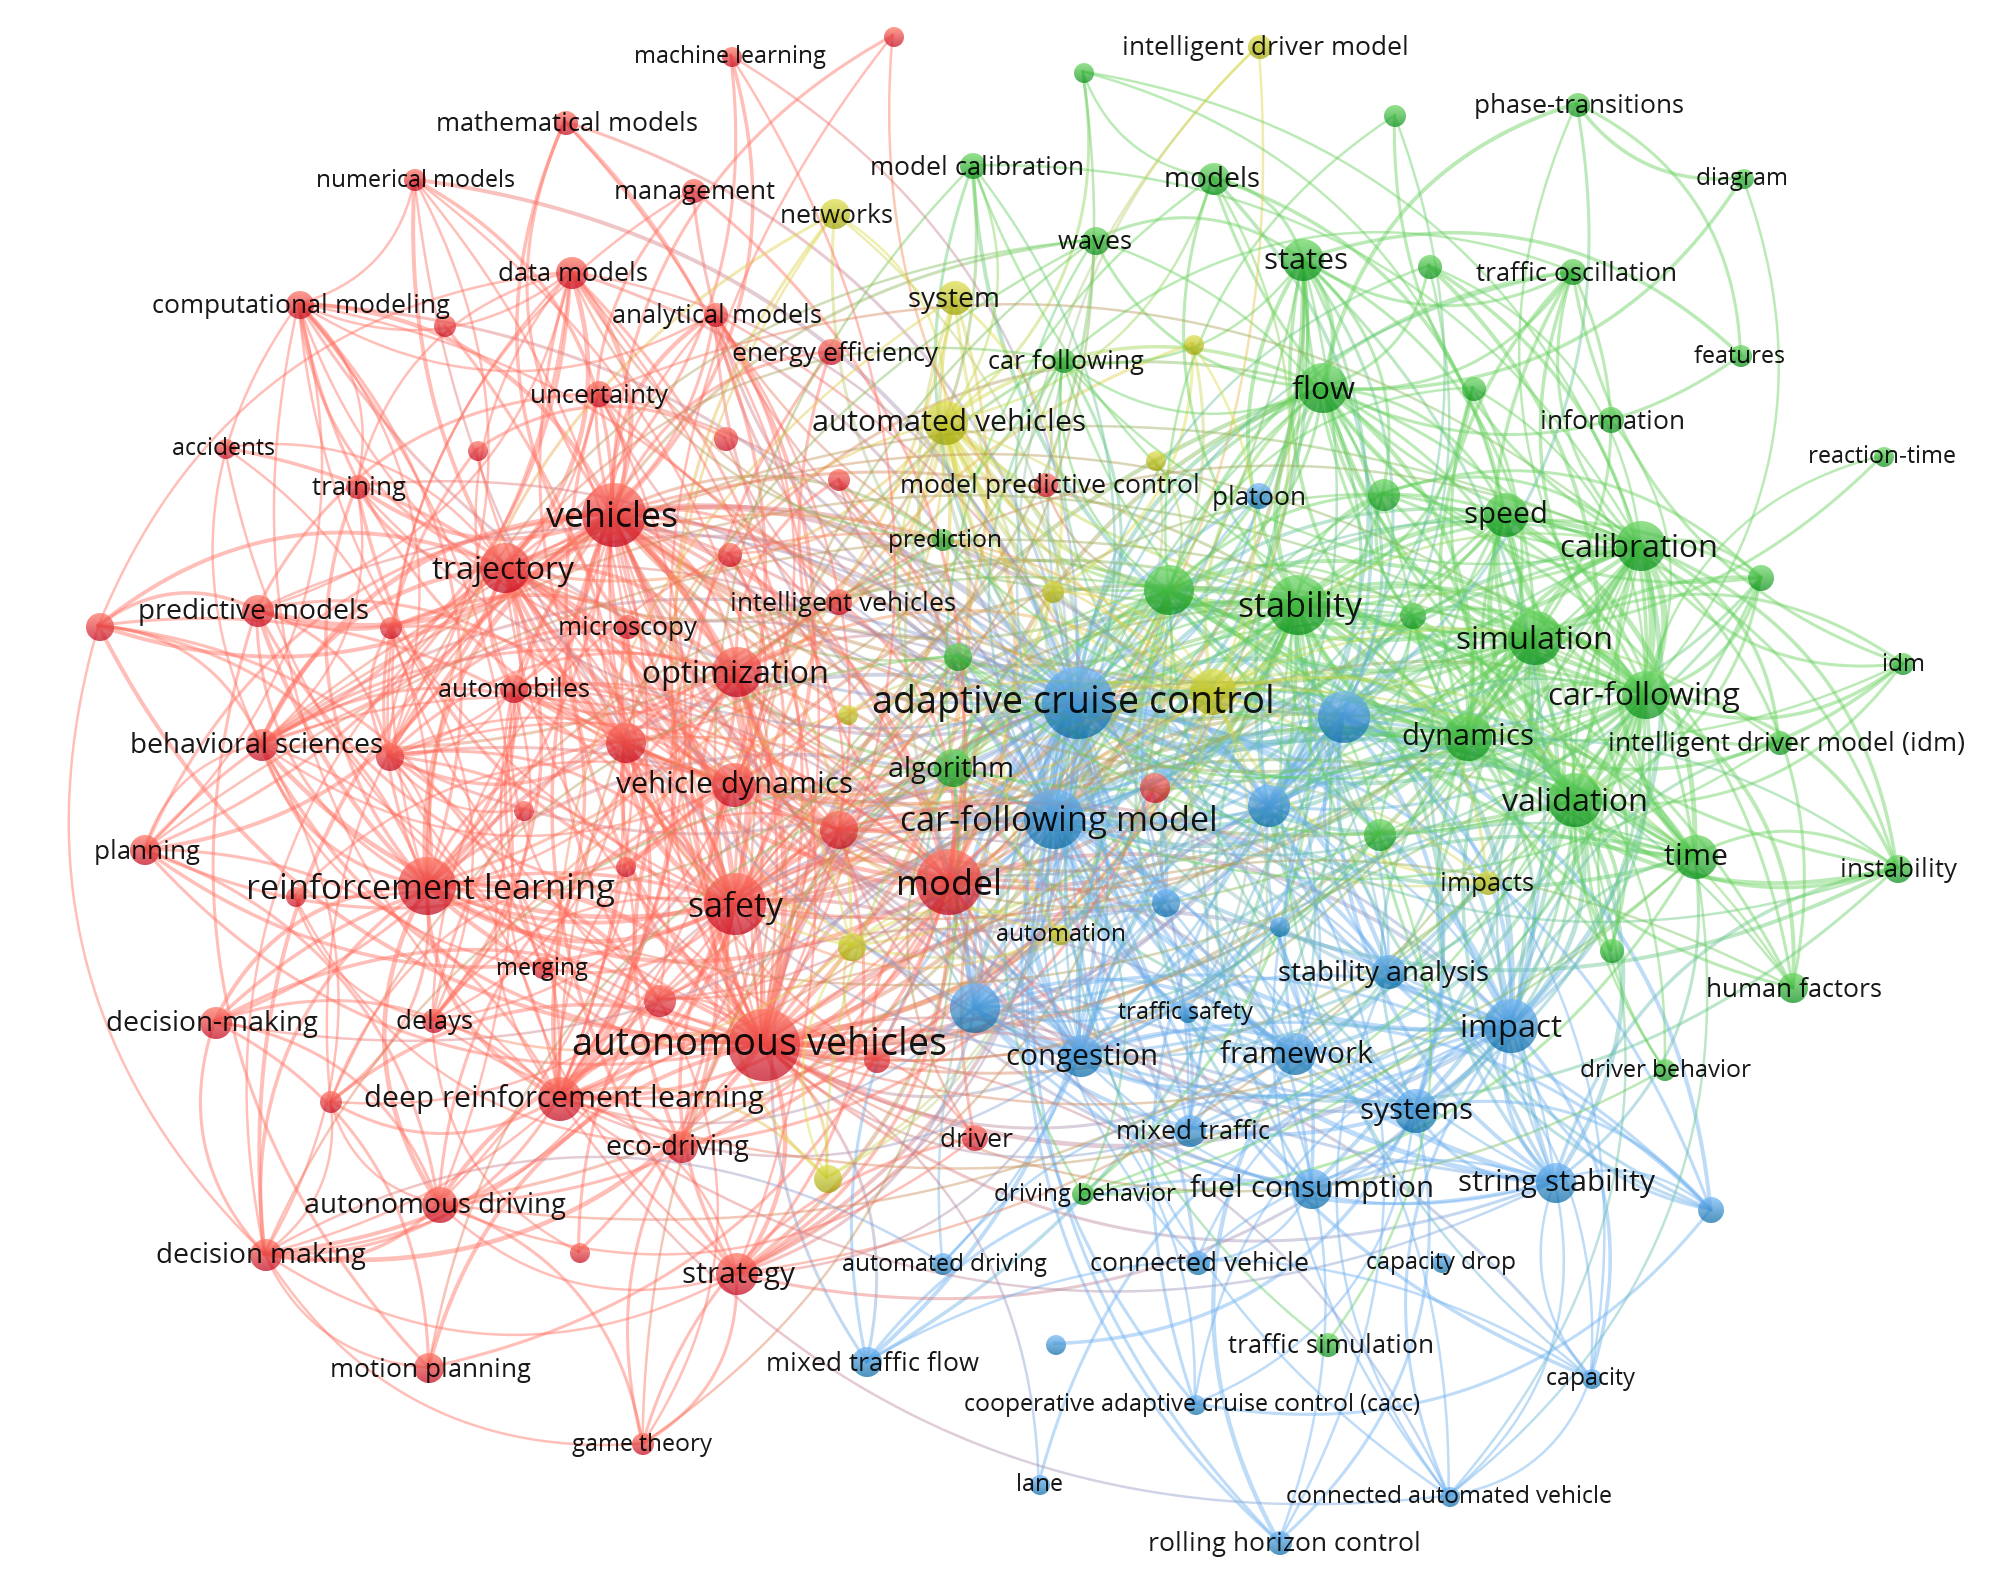
\includegraphics[width=1\linewidth]{Figure/Key.png}
    \caption{Bibilographic coupling of keywords.}
    \label{fig:BibKey}
\end{figure}

Fig. \ref{fig:BibKey} illustrates the bibliographic coupling network of keywords, aiding in identifying research hot-spots in IDM related studies. The size of each solid circle indicates the frequency of a keyword, while the thickness of the connecting lines reflects the co-occurrence between keywords. A total of 1,285 keywords, including both author and index keywords, were analyzed. Using the full-counting method and setting a minimum threshold of 10 papers per keyword, 57 keywords met the criteria. Prominent terms include "autonomous vehicles," "adaptive cruise control," "model," "simulation," "safety," "stability," "reinforcement learning," "optimization," "traffic flow," "vehicle dynamics," "car-following model," "connected vehicles," "validation," "design," "trajectory," "algorithm," and "eco driving."

Building on the bibliometric analysis, we gain a comprehensive overview of IDM research development over the past 25 years. We conducted a cluster analysis of 313 papers, categorizing them into four main areas: basic IDM Overview, theoretical applications of basic IDM, practical applications of basic IDM, and extensions of IDM. The basic IDM overview examines basic attributes, assumptions, and model properties related to traffic theory. Theoretical applications focus on theoretical and calibration uses of IDM. Practical applications cover traffic bottleneck management, section and network control, and interdisciplinary uses. Lastly, extensions of IDM explore physics-based advancements and hybrid models that integrate data-driven and theoretical approaches. The classification is illustrated in Fig. \ref{fig:review}. We will provide a systematic review of IDM-related studies published over the past 25 years based on this classification.

\begin{figure}
    \centering
    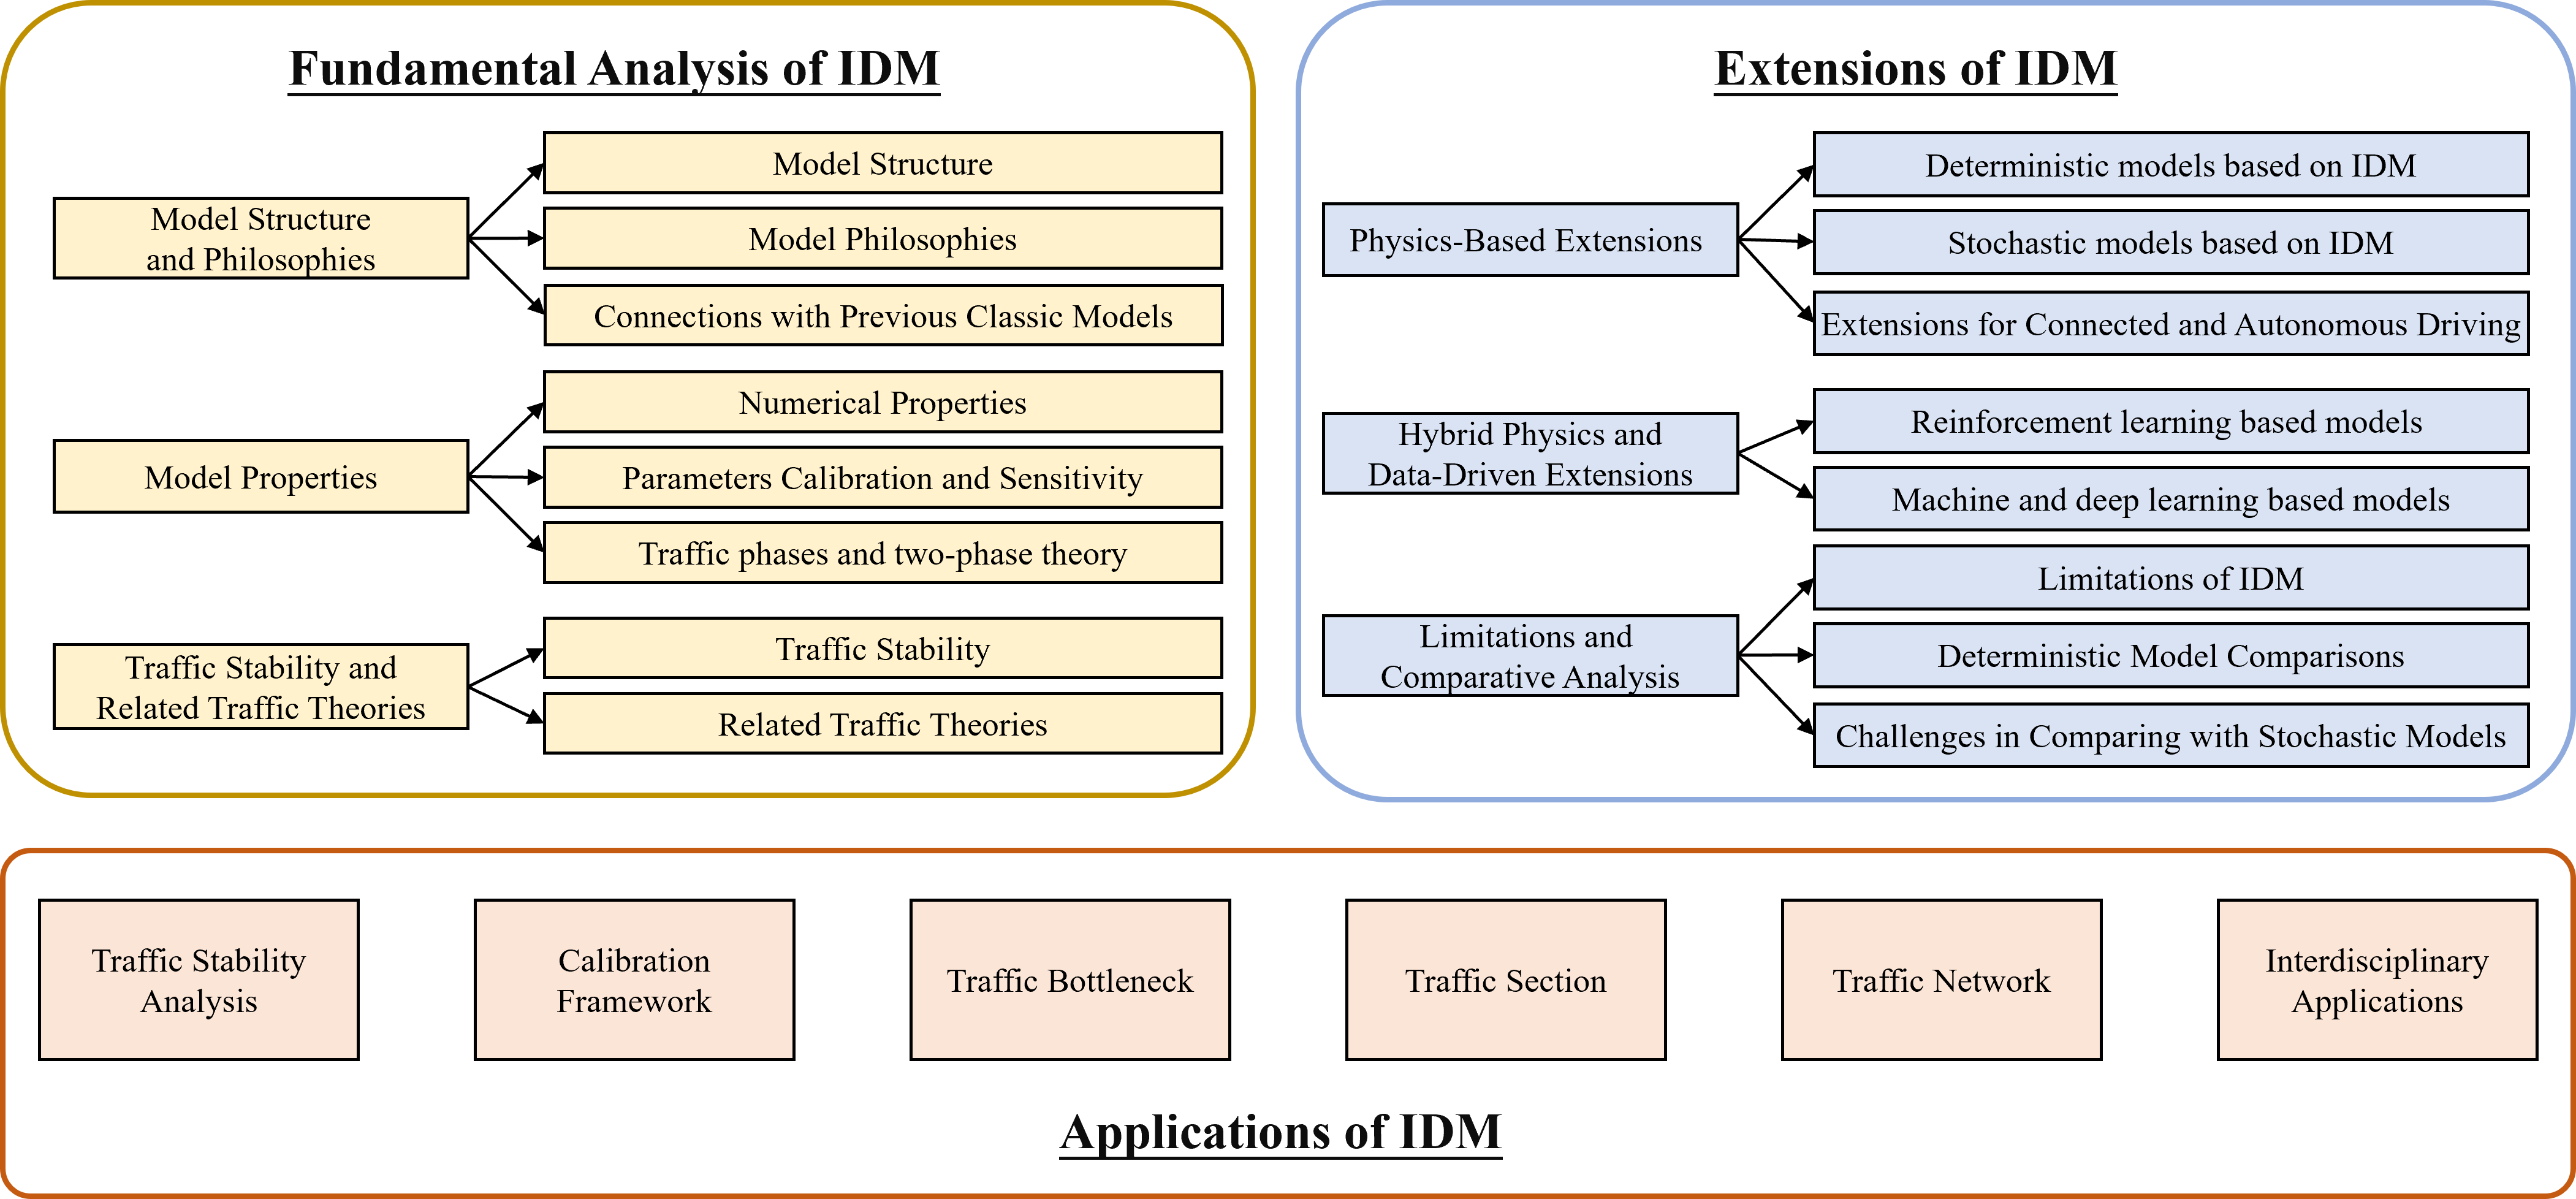
\includegraphics[width=1\linewidth]{Figure/Review.png}
    \caption{Classification of IDM-related literature.}
    \label{fig:review}
\end{figure}

\section{Literature Review}

In this section, the literature is organized into four parts: basic IDM overview, theoretical applications of basic IDM, practical applications of basic IDM, and extensions of IDM. Although some studies span multiple categories, for clarity, we have assigned each study to one primary category in our review. For clarity and ease of reading, we use several abbreviations. Table \ref{tab:abb} provides a list of the frequently used abbreviations along with their full names.

\begin{table}[H]
\centering
\caption{Abbreviations and full names of concepts in IDM-related research.}
\label{tab:abb}
\begin{tblr}{
  hline{1,15} = {-}{0.08em},
  hline{2} = {-}{},
}
Abbreviations & Full names\\
ACC & Adaptive Cruise Control\\
CACC & Cooperative Adaptive Cruise Control\\
HV & Human-driven Vehicle\\
AV & Autonomous Vehicle\\
CV & Connected Vehicle\\
CAV & Connected and Autonomous Vehicle\\
RL  & Reinforcement Learning\\
V2X & Vehicle to Everything\\
FF & Free Flow\\
CF & Car Following\\
MCMC & Markov Chain Monte Carlo\\
VANET & Vehicular Ad-hoc Network\\
VSL & Variable Speed Limits
\end{tblr}
\end{table}

\subsection{basic IDM Overview}

Before conducting a systematic review of the literature on IDM, this section will carefully introduce and summarize its basic features based on the cornerstone research related to the basic IDM, considering that this model is a key tool to capture the dynamics of individual vehicles and a fundamental model of emergent phenomena in traffic systems. We first conduct a formal analysis of IDM to study its mathematical foundations and behavioral assumptions. Next, we will explore traffic fluctuations in IDM to understand how vehicle interactions lead to emergent flow patterns and instabilities. We will also analyze spatiotemporal traffic phases, focusing on the ability of IDM to capture complex traffic phenomena at different temporal and spatial scales. 

\subsubsection{Basic Attributes and Assumptions of IDM}

As outlined in Equations (\ref{equ:IDM1}) and (\ref{equ:IDM2}), the IDM is a nonlinear car-following model characterized by five parameters: $a$, $b$, $v_0$, $s_0$, and $T$. According to \cite{treiberMicroscopicCalibrationValidationCarFollowing2013}, these parameters are intuitive, each is related to a specific driving regime: the desired speed $v_0$ is relevant for cruising in free-flow scenarios, the desired time gap $T$ pertains to steady-state car-following, the minimum gap $s_0$ is associated with creeping and standing traffic, and the maximum acceleration $a$ and desired deceleration $b$ relate to non-steady traffic flow. This design not only makes IDM have strong physical meaning, but also has analytical value. However,  \cite{sharmaMoreAlwaysBetterImpact2019b} found that there is no one-to-one correspondence between IDM parameters and driving regimes. Specifically, the acceleration behavior of the IDM driver in a specific state is controlled by the interaction of multiple IDM parameters.This highlights the importance of considering parameter interactions and dataset characteristics when interpreting IDM calibration results.

In addition to the parameters with obvious physical meanings, IDM also effectively captures the acceleration behavior of drivers by balancing two key components: a non-interaction term and an interaction term. The model defines the desired speed as the maximum attainable speed in free-flow conditions (FF), where drivers can accelerate smoothly to maintain this speed without hindrance. However, in car-following scenarios (CF), the driver's ability to reach the desired speed is constrained by the leading vehicle, although the goal to achieve this speed remains unchanged. The IDM acceleration formula incorporates a non-interaction term, reflecting the driver's acceleration in the absence of external influences, and an interaction term, which accounts for the deceleration required due to the presence of a leading vehicle. In FF conditions, acceleration is primarily determined by the non-interaction term, while in CF conditions, both terms significantly influence the dynamics. The relative weight of these terms in IDM is dependent on the driver's current speed, the speed of the leading vehicle, and the distance between them. These factors collectively ensure that the IDM provides a nuanced and realistic depiction of vehicle dynamics across diverse traffic scenarios.

Hence, IDM is widely used not only because it has a clear physical meaning, but also because it was developed with some basic assumptions built on the modeling philosophy \citep{treiberTrafficFlowDynamics2013}:

\begin{enumerate}
    \item \textbf{Acceleration Conditions}: The acceleration must satisfy specific general conditions to ensure a complete model.

    \item \textbf{Equilibrium Distance}: The minimum safe following distance to the leading vehicle should be no less than a designated "safe distance," calculated as $s_0 + vT$, where $s_0$ is the minimum gap and $T$ is the time gap to the leading vehicle.

    \item \textbf{Braking Strategy}: An intelligent braking approach governs interactions with slower vehicles or obstacles:
    \begin{itemize}
        \item Under normal conditions, braking is gradual, smoothly reducing deceleration to zero as the vehicle approaches a steady state or stops.
        \item In critical situations, the deceleration exceeds comfortable levels until safety is restored, after which it resumes normal deceleration.
    \end{itemize}

    \item \textbf{Smooth Mode Transitions}: Transitions between driving modes, such as from acceleration to car-following, are smooth. The model ensures that the jerk, or the derivative of acceleration, remains finite, indicating continuous differentiability across variables.

    \item \textbf{Model Parsimony}: The model should be as simple as possible, with each parameter intuitively representing a specific aspect of driving behavior, aiding in effective calibration and interpretation.
\end{enumerate}




\subsubsection{Model Properties and Related Traffic Theory}


Based on the IDM, a series of work on the its properties under the CF models framework have been conducted. As to the integration scheme, \cite{treiberComparingNumericalIntegrationSchemes2015} find the ballistic update always prevails Euler’s method although both are of first order after comparing four explicit methods: Euler’s method, ballistic update, Heun’s method (trapezoidal rule), and the standard forth-order Runge-Kutta. \cite{treiber_delays_2006} studied the effects of limited reaction time, estimation error, and multi-anticipative effects. The unstable effect of the reaction time and estimation error can be compensated through space and time anticipation.\cite{treiberMicroscopicCalibrationValidationCarFollowing2013} explored methodologies for calibrating CF models based on IDM. They emphasized criteria for assessing model quality in addition to RMSE, including completeness, robustness, parameter orthogonality, and intuitive parameters aligned with plausible values. The study highlighted that global calibration based on gaps is more reliable than local calibration or those based on speeds or accelerations. Moreover, they found that a sampling rate of 1 Hz suffices, with data completeness and a minimum interval of 300 seconds being crucial for accurate calibration, while data smoothing had minimal impact. \cite{yangClassificationUnificationMicroscopicDeterministic2015a} proposed one universal mathematical structure in microscopic traffic models and proved that IDM is equivalent to a generalized Optimal Velocity (OV) model . 

From the aspects of traffic mechanism, the properties of IDM are also investigated. traffic flow instabilities, known as stop-and-go waves, arise from delays in drivers adjusting their speed to actual conditions and may lead to traffic oscillations. These oscillations occur when drivers repeatedly decelerate and accelerate instead of maintaining a steady pace. Such fluctuations are critical because they detrimentally affect traffic efficiency and safety. They result in longer travel times, increased fuel consumption, and higher emissions due to the constant speed changes. Furthermore, these oscillations can propagate backward through traffic, worsening congestion and potentially leading to traffic jams. \cite{treiberTrafficFlowDynamics2013} has proved that IDM can reproduce the convective instability propagating upstream, linear convective instability propagating downstream which is destroyed by nonlinearities, and of the limit between convective and absolute instability. \cite{treiberEvidenceConvectiveInstabilityCongested2011} provided evidence that the concept of convective instability is relevant to the instability of traffic congestion. \cite{jiangTrafficExperimentRevealsNature2014a} revealed that the oscillation of a platoon shows a concave growth pattern, i.e., the standard deviation of vehicle acceleration increases in a concave shape as the vehicle moves upstream in the platoon. However, the oscillation of IDM is in a convex way. This promotes the improvement and development of IDM.

\begin{figure}
        \centering
        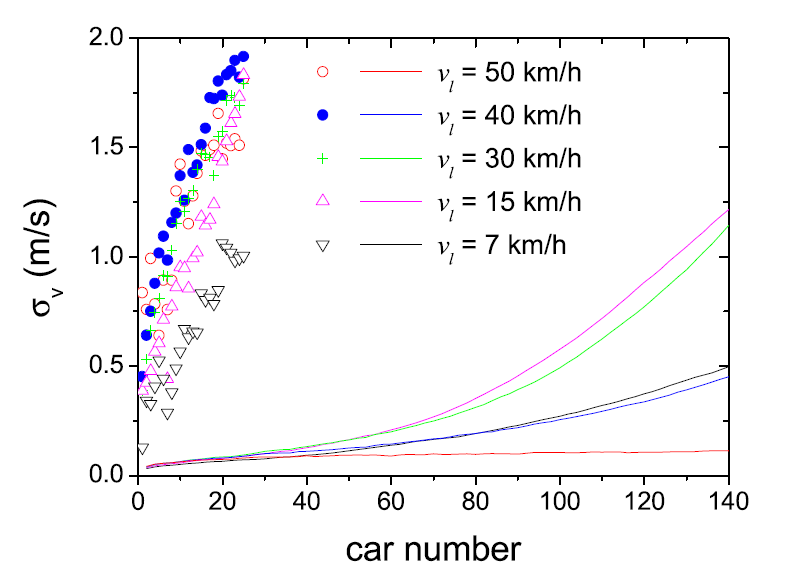
\includegraphics[width=0.5\linewidth]{Figure/IDM_Growth.png}
        \caption{Simulation results (solid lines) of the standard deviation $\sigma_v$ of the time series of the velocity of each car of IDM from \cite{jiangTrafficExperimentRevealsNature2014a}.}
        \label{fig:IDMGrowth}
    \end{figure}

As a representative of classic CF models, IDM has inherent differences from the models derived from three-phase traffic theory \citep{kernerFailureClassicalTrafficFlow2016}. This arises from different definition of the traffic phases. IDM belongs to the two-phase models would additionally produce oscillatory traffic states such as wide moving jams or stop-and-go waves. It have been proved to reproduce five congested traffic patterns, namely pinned localized clusters (PLC), moving localized clusters (MLC), triggered stop-and-go waves (TSG), oscillating congested traffic (OCT), and homogeneous congested traffic (HCT). The OCT and TSG patterns look somewhat similar, and there is no discontinuous transition between these patterns. \cite{treiberMemoryEffectsMicroscopicTraffic2003} utilized the Intelligent Driver Model (IDM) for simulation and demonstrated that the non-instantaneous adaptation of driving behavior to traffic conditions, when combined with the conventional method of measuring flow-density data, can explain the observed inverse-$\lambda$ shape and the wide scattering of flow-density data in "synchronized" congested traffic. Furthermore, the fundamental diagram in \citep{treiberUnderstandingWidelyScatteredTraffic2006} highlights the presence of free, synchronized, and jammed traffic states, along with a wide scattering in the congested traffic regime. While in the three phase traffic theory, \cite{kernerPhysicsTraffic2004}, another traffic state has been introduced, so-called synchronized flow, which is characterized by a self-generated scattering of the traffic variables. \cite{treiberThreephaseTrafficTheoryTwophase2010} claim that if the model parameters are suitably chosen, the conceptionally simpler two-phase models can display all stylized facts mentioned in three-phase theory. More details can be found in \cite{kernerPhysicsTraffic2004} and \cite{treiberTrafficFlowDynamics2013}.

\begin{figure}
    \centering
    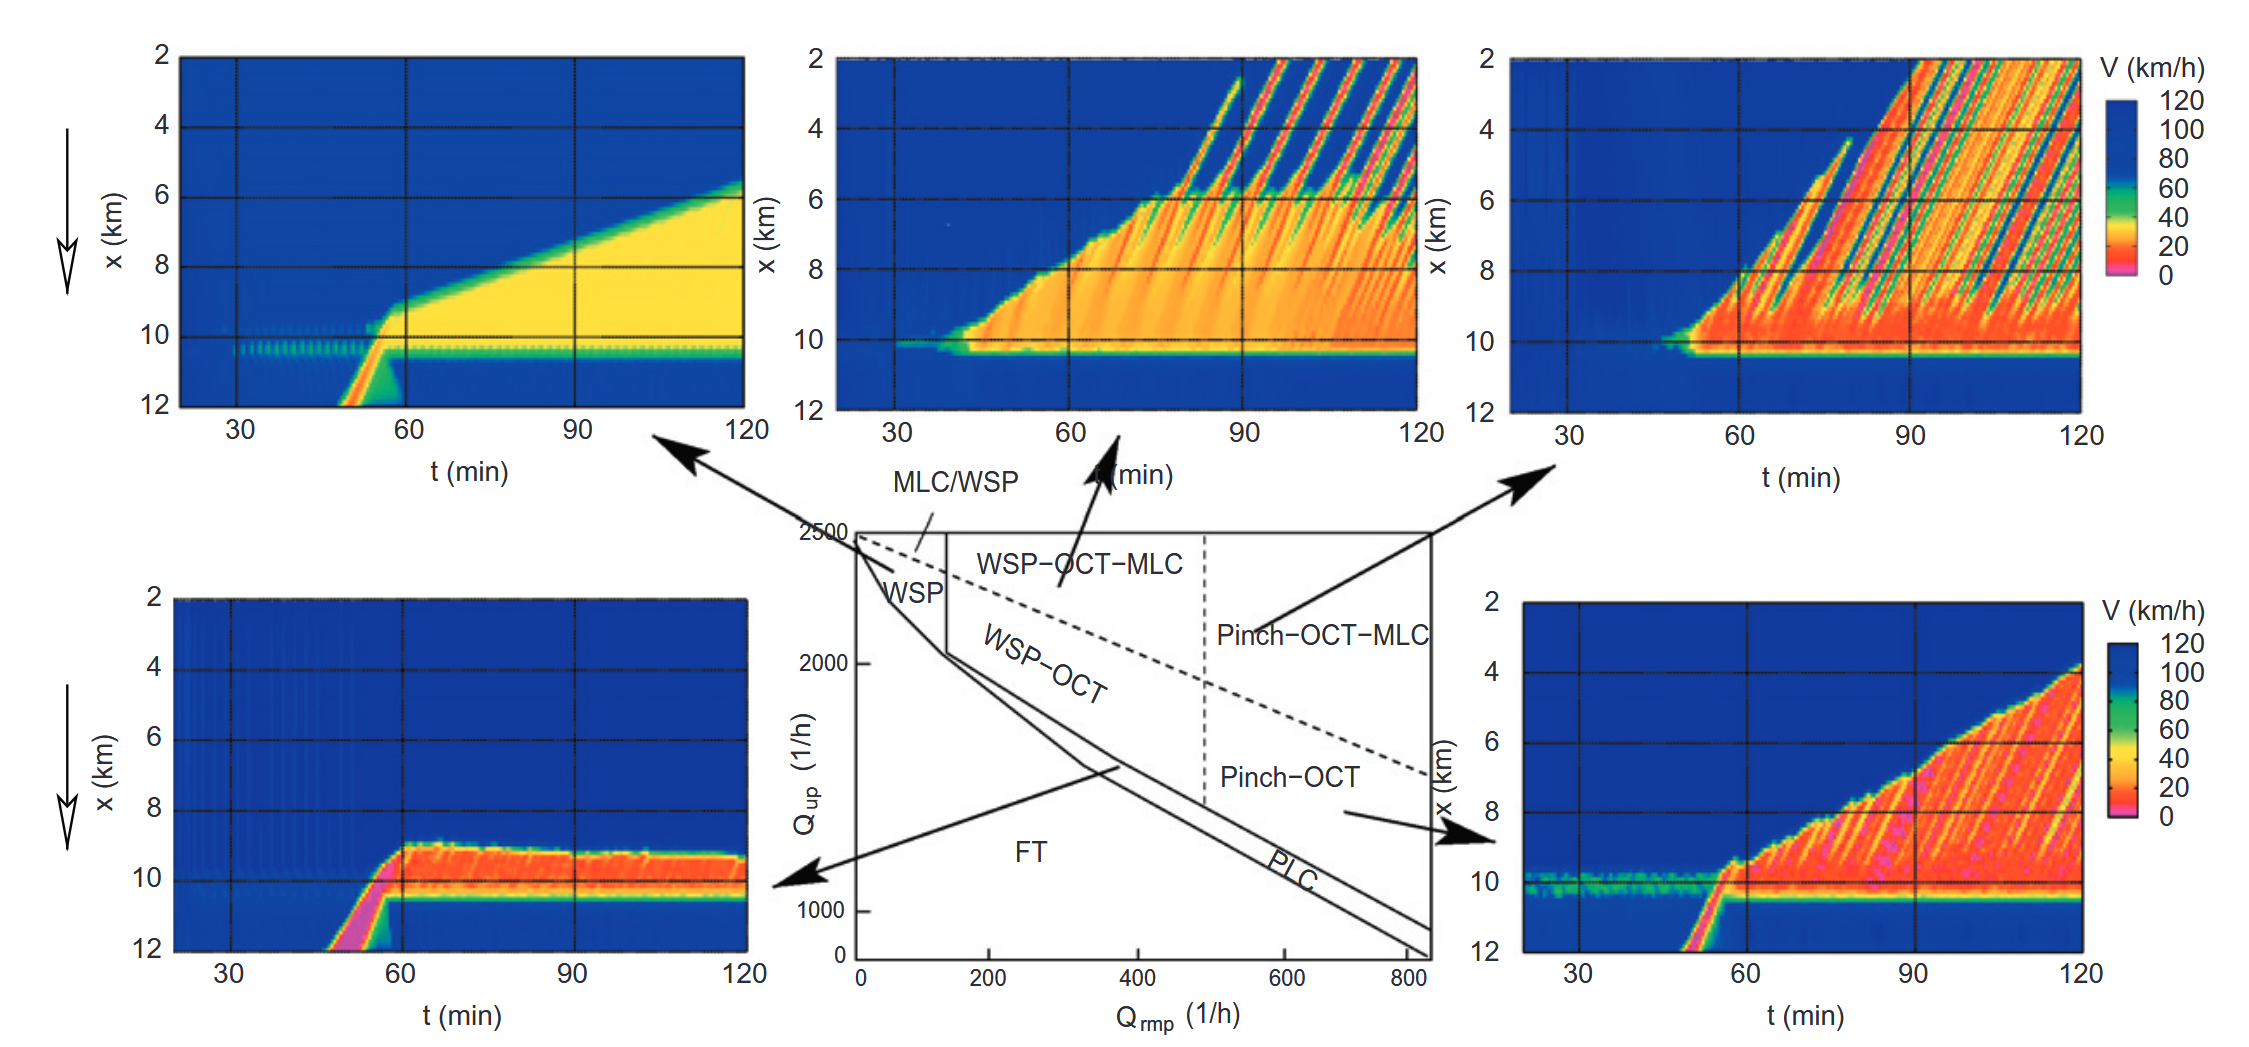
\includegraphics[width=0.75\linewidth]{Figure/IDMTP.png}
    \caption{Dynamic phase diagram of on-ramp-induced congested traffic patterns simulated by IDM from \cite{treiberThreephaseTrafficTheoryTwophase2010}.The abbreviations denote free traffic (FT), pinned localized cluster (PLC), moving localized cluster (MLC), homogeneous congested traffic (HCT), oscillatory congested traffic (OCT), and triggered stop-and-go (TSG) pattern.}
    \label{fig:enter-label}
\end{figure}

\subsection{Theoretical Applications of basic IDM}

This section reviews the direct theoretical analysis of the basic IDM. As a widely studied model, IDM has been used to derive the stability of various traffic flow systems and to test various aspects of various traffic flow research frameworks such as calibration frameworks. These contributions are both theoretical and foundational.


\subsubsection{Theoretical Utilizations}

IDM, recognized for its highly non-linear nature, poses challenges for theoretical analysis. Its primary applications are found in the derivation of fundamental diagrams and stability analysis. \cite{yao_modeling_2023} leveraged IDM to explore the fundamental diagram of mixed traffic flows with dedicated lanes for CAVs, evaluating traffic capacity under various conditions. Concurrently, \cite{gao_predictive_2023} developed a macro fundamental diagram model of intersections based on IDM and applied shock wave theory to predict intersection queue lengths and dissipation times.

A significant focus has been on understanding traffic stability through IDM. \cite{kestingHowReactionTimeUpdate2008} initiated this exploration by analyzing the influence of reaction time and speed adaptation on traffic stability, using IDM to uncover various instability mechanisms. Building on this, \cite{jinEquivalenceContinuumCarFollowingModels2016a} demonstrated the equivalence between continuum and car-following models, illustrating that higher-order IDM can be transformed into continuous models with consistent stability conditions. \cite{monteil_linear_2014} advanced the discussion by examining string stability in mixed traffic flows and the impact of multiple anticipations in cooperative car-following models. \cite{montaninoHomogeneousHeterogeneousTrafficFlows2021b} further delved into string stability in mixed and heterogeneous traffic flows, incorporating uncertainties in model parameters. They later proposed a unified modeling framework \citep{montaninoStringStabilityMixedHeterogeneous2021b} to assess stability, considering driver and vehicle heterogeneity and using IDM to verify this framework. \cite{bouadiStochasticFactorsStringStability2022b} extended these concepts into the realm of stochastic models, investigating string stability in stochastic car-following models using IDM with stochastic variants and the generalized Lyapunov equation to establish stability conditions.


\subsubsection{Calibration Analysis }

Research on IDM-based calibration can be categorized into several key areas. Firstly, the development of calibration frameworks focuses on effectively handling Model Performance (MoP), Goodness of Fit (GoF), and trajectory completeness. Secondly, model evaluation involves calibrating various car-following models to compare their performance across different metrics. Thirdly, algorithm design aims to create efficient optimization algorithms for calibration processes. Lastly, behavior feature extraction uses IDM-calibrated data to classify different driving behaviors and vehicle types. 

For the development of calibration frameworks, building on this focus on error, \cite{jin_reducing_2014} explored error accumulation in car-following models calibrated with vehicle trajectory data, deriving a dynamic error model based on acceleration. \cite{longBiScaleCarFollowingModelCalibration2024a} introduced a bi-scale car-following model calibration using corridor-level trajectories, highlighting macro measurement error accumulation. To address the validation aspect, \cite{treiberValidationTrafficFlowModels2012} developed a quantitative method for calibrating and validating traffic flow models based on the spatiotemporal evolution of congested traffic patterns. In terms of parameter importance and simplification, \cite{punzo_we_2015} conducted sensitivity analysis on driving behavior models, finding leader trajectory more important than parameters, and proposed a simplified model with faster convergence. For setting robust calibration objectives, \cite{punzoCalibrationCarFollowingDynamicsAutomated2021} proposed robust guidelines for selecting MoP and GoF for calibrating car-following dynamics using Pareto efficiency and indifference curves for function comparison. Focusing on data integrity, \cite{sharmaMoreAlwaysBetterImpact2019b} investigated the impact of vehicular trajectory completeness on the calibration and validation of car-following models. Finally, addressing behavioral pattern recognition, \cite{zhengMultiObjectiveCalibrationFrameworkCapturing2023b} proposed a multi-objective calibration framework to capture behavioral patterns of autonomously-driven vehicles, validating with empirical observations of ACC vehicle dynamics.


As for the development of the optimization algorithms for calibration, \cite{rahman_improving_2015} proposed a stochastic calibration method using Bayesian estimation and MCMC simulation. \cite{liGlobalOptimizationAlgorithmTrajectory2016b} developed a global optimization algorithm combining direct and gradient searches for car-following models. \cite{zhongCrossEntropyMethodProbabilisticSensitivity2016b} introduced a calibration method using the Cross-Entropy Method and sensitivity analysis under noisy data.\cite{fardCopulaBasedEstimationDistributionAlgorithm2019b} suggested a copula-based algorithm to explore complex parameter interactions in traffic models.\cite{wangIntegratedSelfConsistentMacroMicroTraffic2024a} created an integrated macro-micro calibration framework using enhanced optimization and deep learning.

In addition to the above theme, calibration is crucial for model evaluation. \cite{zhuModelingCarFollowingBehaviorUrban2018b} investigated the applicability of car-following models for Chinese drivers, highlighting IDM's effectiveness and portability on Shanghai highways. \cite{campi_roundabouts_2024} assessed various models in roundabout scenarios, with IDM excelling in capturing CAV behavior. \cite{zhouExperimentalFeaturesEmissionsFuel2023b} used four classical emission and fuel consumption models and found IDM effective at the vehicle pair level for energy consumption and emissions predictions. However, at the platoon level, predicted results were almost constant, contrasting with experimental observations.

Based on calibrated IDM, different behavior patterns and vehicle types can be extracted. \cite{ossenHeterogeneityCarFollowingBehaviorTheory2011b} used data collected by helicopter to calibrate the IDM to identify differences in following behaviors between different driver types, showing significant heterogeneity. \cite{makridis_response_2020} estimated the response time of vehicles equipped with ACC by calibrating IDM parameters and found that it was comparable to that of human drivers. \cite{hu_autonomous_2023} calibrated IDM parameters to distinguish the empirical following behaviors of AVs and HVs in Waymo data. \cite{li_automated_2023} proposed an AV identification algorithm based on IDM calibration results, that is, using error results to distinguish AVs from HVs.

\subsection{Practical Applications of basic IDM}

This section reviews the practical applications which are categorized by different layers across various traffic scenarios. At the bottleneck level, it includes intersection trajectory planning and ramp merging control. At the road segment level, it covers integrated lateral and longitudinal control, mixed traffic flow analysis, and monitoring of road conditions and communication errors. At the network level, it discusses route planning and signal optimization. Additionally, other applications include AV safety testing and miscellaneous tasks such as trajectory restructuring, communication algorithms, and network attack simulations. 

\subsubsection{Applications in Traffic Bottleneck Management and Control}

Next, we will focus on two typical bottlenecks, intersections and ramps, and summarize the IDM-related research in the field of traffic bottlenecks from the aspects of intersection system evaluation, vehicle trajectory planning and signal optimization, and ramp merging management.

\paragraph{\textbf{intersection systems:Evaluation, Vehicle trajectories planning and signal optimization}}
Intersection research mainly includes evaluation of the intersection system, vehicle trajectory planning and signal optimization research, as well as the coordinated optimization research of the two.\cite{joererVehicularNetworkingPerspectiveEstimating2014a} introduced a method to evaluate vehicle collision probability at intersections, using modified traffic simulators based on IDM to assess intelligent transportation system safety, especially when traffic rules are disregarded. \cite{schrader_global_2024} employed Sobol global sensitivity analysis to identify how simulation input parameters like IDM's parameter impact performance metrics of the intersection system. For vehicle trajectory planning related research, IDM is mainly used as a simulation model for background vehicles or manually driven vehicles \citep{chen_human-like_2023,dong_comparative_2022,ghosh_traffic_2022,guoCoordinationConnectedAutomatedVehicles2023a,jiangEcoApproachingIsolatedSignalized2017a,medina_cooperative_2018,stebbinsCharacterisingGreenLightOptimal2017a,wang_learning_2023,xiaoDecisionMakingAutonomousVehiclesRandom2024a,zhangPlatoonCenteredControlEcoDrivingSignalized2023b,zhang_risk-aware_2023}.In addition,\cite{zhouCooperativeSignalFreeIntersectionControl2022b} used IDM as the microscopic simulation model for CAV under the corporative intersection control framework. For the signal optimization, IDM is also used as the simulation foundation \citep{cao_gain_2022,sohn_waterfilling_2023,yang_enhancing_2024}. \cite{duCoupledVehicleSignalControlMethod2021b} developed an efficient coupled vehicle signal control method for optimizing traffic signal timing and CAV trajectories in mixed traffic environments, using IDM as the artificially driven vehicle model. \cite{huang_reservation-based_2023} proposed a reservation-based cooperative ecological driving model for optimizing CAV trajectories and intersection signals at isolated intersections, using background vehicles simulated by IDM. \cite{liEcoDrivingSystemElectricVehicles2018a} integrated an electric vehicle eco-driving system and signal control in a V2X environment, using IDM to formulate non-connected electric vehicle following rules and a hybrid algorithm for optimization. \cite{liang_equitable_2020} combined connected vehicle technology for traffic signal control at isolated intersections, optimizing platoon dissipation based on IDM estimation of vehicle proximity.

\paragraph{\textbf{Ramp merging:}}
For ramp scenarios, the main focus is on research related to collaborative merging. \cite{baselt_merging_2014,chen_deep_2023,hou_cooperative_2023,ito_coordination_2019,maProgressiveVirtualRiskBasedVehicle2024a,tangNovelHierarchicalCooperativeMerging2022b,xiongManagingMergingCAVLane2022b,zhou_state-constrained_2019} proposed various corporative merging methods by using IDM to simulate a HV in a mixed traffic merging scenario.\cite{guNetworkTrafficInstabilityAutomated2022b} use macroscopic or network fundamental diagrams  to study the impact of CAVs on network flow destabilization caused by turning and merging maneuvers. They used IDM, Human Driving Model(HDM) and cooperative IDM to simulate the AV, HV and CAV, respectively. \cite{silgu_combined_2022}  proposed a controller integrating ramp metering and variable speed limits for freeway traffic, tested via SUMO simulations with CACC and HVs.  For the system evaluation of ramp, \cite{xiaoUnravellingEffectsCooperativeAdaptive2018a} analyzed the impact of CACC deactivation on traffic flow at merging bottlenecks, using simulations to evaluate capacity and queue discharge rates.

\subsubsection{Applications in Section and Network  Control}

Among the research related to the direct application of IDM, the vehicle control especially under the connected and autonomous environment is most popular. We divide these literature into four types: individual longitudinal control (car following),
Individual lateral control (lane change), integration of individual lateral and longitudinal coordinated control.

\paragraph{\textbf{Vehicle longitudinal and lateral control:}}
In individual longitudinal control, scholars tend to design the control algorithm of the automatic vehicle based on physical methods or data-driven methods. Therefore, IDM is still used as a vehicle control model for background vehicles, ACC vehicles, manually driven vehicles or some low-connectivity scenarios \citep{juPredictiveCruiseControllerElectric2023a,kamal_efficient_2016,kamalLookAheadDrivingSchemesEfficient2022a,li_deep_2022,li_effect_2015,liu_semantic_2023,liu_potential_2023,liuSpatiotemporalTrajectoryPlanningAutonomous2024a,luLearningDriverSpecificBehaviorOvertaking2018a,ma_energetic_2022,maPersonalizedDrivingBehaviorsFuel2022a,manolis_real_2020,shiConnectedAutomatedVehicleCooperative2021b,shiDeepReinforcementLearningBased2023b,suo_model-free_2024,tangHighwayDecisionMakingMotionPlanning2022a,tas_making_2018,toghi_social_2022,valiente_prediction-aware_2024,wegener_automated_2021,wuFlowModularLearningFramework2022a,wu_hybrid_2023,yan_unified_2023,yangIsolatedIntersectionControlVarious2016a,yuAssessmentDynamicPlatoonInformation2023a,yuanPredictiveEnergyManagementStrategy2019,zhang_stackelberg_2024,zhangNoMoreRoadBullying2023a,zhou_development_2020,milanesModelingCooperativeAutonomousAdaptive2014b,fernandes_platooning_2012,vivekCyberphysicalRisksHackedInternetconnected2019a}. Among these, \cite{zhangNoMoreRoadBullying2023a} and \cite{manolis_real_2020} integrated the IDM into the simulation software VISSIM and AIMSUN, respectively.

Compared with longitudinal control, there are relatively few studies on lateral control, and IDM is generally used as a longitudinal control model to study how to perceive, cooperate, make decisions, and adjust in lane change decisions base on the methodologies of game theory, model predictive control, reinforcement learning and etc. like \citep{chen_adversarial_2022,gongGameTheoryBasedDecisionMakingIterative2023a,guIntegratedEcoDrivingAutomationIntelligent2022a,hwang_autonomous_2022,li_bounded_2024,liuMultistepCooperativeLaneChange2024a,liu_interaction-aware_2023,scheel_recurrent_2022,sheng_cooperation-aware_2023,sunberg_improving_2022,wangModelingBoundedRationalityDiscretionary2022a,zhang_game_2020}.

For the individual lateral and longitudinal coordinated control, research usually integrate two types of models into one unified framework \citep{kanagaraj_self-driven_2018,li_developing_2023,mullakkal-babu_hybrid_2021}.

\paragraph{\textbf{Evaluation of CAV systems on road section:}}
In the road section scale, many research focus on evaluate the performance of the CAV systems. For example,several research evaluate the stability and the capacity of this system \citep{qin_analytical_2021,qinStabilityAnalysisConnectedVehicles2023a,sunStabilityExtensionCarFollowingModel2023b,sunRelationshipCarFollowingString2020b,shang_impacts_2021,talebpourEffectInformationAvailabilityStability2018a,talebpourInfluenceConnectedAutonomousVehicles2016a,wang_stability_2019,yao_linear_2021,zhou_analytical_2021}. \cite{alhariqiImpactVehicleArrangementMixed2023a,zhou_modeling_2020} evaluated the impact of different following arrangements in a platoon on the road emissions.\cite{mullakkal-babu_comparative_2022} evaluated the adverse impact of takeover behavior on mixed traffic flow at different takeover time levels for fully automated vehicles.\cite{rahman_longitudinal_2018} explored the impact of CV platooning on highways on longitudinal traffic safety at different market penetration rates, and studied the role of the allocation of CV (i.e., whether they are limited to specific lanes) on traffic safety.\cite{wangEgoEfficientLaneChangesConnected2022a} studied the impact of lane change on the sytem.\cite{wuTimeDependentPerformanceAnalysis80211pBased2020a} investigated the impact of disturbances caused by acceleration and deceleration of the lead vehicle, gusts, and uncertainties in the platoon control system, such as aerodynamic drag and rolling resistance torque, on platoon communication.
\cite{yao_fuel_2021} studied the impact of CAVs on fuel consumption and emissions of mixed highway traffic flows. \cite{yaoAnalysisImpactMaximumPlatoon2023a} explored the impact of the maximum size of an autonomous platoon on mixed traffic flows. \cite{zhou_impact_2021} studied
the impact of degradation of CAV platooning control modes on the fundamental diagram. Autonomous driving car testing is an important part of autonomous driving research and development, and IDM also plays an important role in this as the background vehicle \citep{sun_scenario-based_2022,li_scegene_2022,sun_adaptive_2022,cao_autonomous_2023,zhang_accelerated_2024,zhang_bayesian_2024}. 

\paragraph{\textbf{Traffic optimization of road section:}}


Furthermore, some system management research on the road section have been conducted. Some tried to improve the traffic capacity of road section based on platoon control.  Most of them use IDM for simulating the HV like \cite{ferreira_impact_2012,ge_optimal_2017,heEcoDrivingAdvisoryStrategiesPlatoon2018a,liu_joint_2022,montaninoTrajectoryDataReconstructionSimulationBased2015b,wangRollingHorizonControlFramework2014b,wang_optimal_2022,wang_trajectory_2022}, while other platoon control related research always use IDM as the degradation model of CAV. Some use the VSL to optimize the CAV system in which IDM is used to simulate HV or CAV \citep{khondakerVariableSpeedLimitMicroscopic2015a,li_developing_2022,li_integrated_2017,luTD3LVSLLaneLevelVariableSpeed2023a,othman_analysis_2022}. \cite{mahajan_improving_2024,schakel_improving_2014} proposed a speed-based lane guidance system and a new on-board advisory system, respectively, to provide recommendations on lanes, vehicle speeds, and headway, optimizing lane allocation under high-traffic conditions to reduce capacity degradation. \cite{wang_cooperative_2020} studied a cooperative ecological driving system for signal corridors, where the CAV switches between a leading vehicle and a following vehicle, and IDM is used to simulate a CAV with network communication failure.

\paragraph{\textbf{Traffic optimization of network:}}
On the road network scale, \cite{huang_characterizing_2023} considered different signal control schemes and demand loading patterns, and focused on the overall network level to consider the traffic flow patterns brought about by autonomous driving mixed traffic. \cite{claes_decentralized_2011} proposed a distributed vehicle path planning method based on predictive information.

\subsubsection{Interdisciplinary Applications}

 IDM is widely recognized for its versatility across numerous research domains beyond its core application in traffic modeling and management of road segments and networks. IDM finds extensive use in areas such as vehicle self-organizing networks, communication algorithms and their associated network attacks within vehicular communications, and even in civil engineering for studies related to bridge loads.

\paragraph{\textbf{Applications in vehicle communications:}}

In the context of vehicular networks,  \cite{wangOptimalFeedbackControlLaw2023a} and \cite{wang_analytical_2024} have significantly advanced the understanding of cyberattacks on automated vehicles by developing an optimal feedback control law and a comprehensive framework for modeling attacks on adaptive cruise control vehicles. \cite{dongDynamicManagerSelectionAssisted2022a} introduced a resource allocation algorithm for 5G-V2X platoons, optimizing communication performance under finite block length constraints, crucial for ensuring ultra-reliable low-latency communications. \cite{jiaDisturbanceAdaptiveDesignVANETenabledVehicle2014a} and \cite{jiaNetworkConnectivityPlatoonBasedVehicular2014a} delved into VANET-enabled platoon architectures, emphasizing disturbance adaptation and network connectivity, which are vital for effective safety message transmission under varying system parameters. Moreover,  \cite{segataAutomaticEmergencyBrakingRealistic2013a} assessed the integration of automatic emergency braking systems within VANETs, while \cite{tianSelfOrganizedRelaySelectionCooperative2017a} proposed a decentralized relay selection algorithm based on non-cooperative game theory to enhance cooperative dynamics. 


\paragraph{\textbf{Applications in civil engineering:}}
 \cite{ge_intelligent_2022} introduced an advanced traffic flow load monitoring system that integrates machine vision and weigh-in-motion  systems, leveraging deep learning for precise vehicle detection and extraction of key parameters for traffic flow load simulation.  \cite{zhou_hybrid_2024} proposed a two-step Hybrid Virtual-Real Traffic Simulation method to replicate the spatiotemporal distribution of bridge loads, demonstrating the broad applicability of IDM in various interdisciplinary fields.


\subsection{Extensions of IDM}


In this section, we explore the extensions of IDM in both physics-based and data-driven approaches, as well as the concept of hybrid models. Physics-based extensions rely on fundamental principles of mechanics and dynamics, capturing the underlying laws of motion to simulate traffic behavior. These models  often  provide insights into the physical interactions within traffic systems. In contrast, data-driven extensions utilize statistical and machine learning techniques to analyze and predict driving patterns based on empirical data. These models are typically more adaptable to real-time changes and can manage complex datasets to improve prediction accuracy. Hybrid models integrate both physics-based and data-driven methods, leveraging the strengths of each to enhance model robustness and performance, offering a more comprehensive approach to capturing the intricacies of traffic dynamics.
 
\subsubsection{Physics-Based Extensions}

The development of IDM extensions for modeling driver behavior has seen significant incremental advancements. These models, based on IDM, can be categorized into two types: deterministic IDM family and stochastic IDM family.

For deterministic models, \cite{kestingAdaptiveCruiseControlDesign2008} expanded IDM to mimic the acceleration of ACC vehicles (IDM-ACC). \cite{li_evaluating_2017,li_evaluation_2017} utilized IDM-ACC to evaluate the impact of the CACC system and the longitudinal driver assistance system on highway rear-end collision risk reduction. Additionally, \cite{li_stability_2015} incorporated power cooperation into IDM, enhancing traffic flow stability under open boundary conditions by proportionally boosting vehicle power based on the leading car. \cite{sarkar_microscopic_2020} developed the Modified IDM (MIDM) using a two-step microscopic model to address heterogeneous traffic flow, enhancing vehicle movement based on potential directions. Concurrently, \cite{saifuzzamanIncorporatingHumanFactorsCarFollowingModels2014c} introduced the Task-difficulty IDM (TD-IDM), integrating human factors by focusing on task difficulty as defined by the Task-Capability Interface model. \cite{chen_sigmoid-based_2024} tackled excessive acceleration in traffic oscillations with the Sigmoid-IDM, employing a Sigmoid function to address car-following failures in free flow. Building on this, \cite{chen_two-dimensional_2024} proposed a two-dimensional lane changing framework inspired by the social force model, incorporating concepts of lane force and gap force.

On the stochastic side, \cite{jiangTrafficExperimentRevealsNature2014a} explored the two-dimensional extension of IDM (2D-IDM), revealing the concave growth pattern of traffic oscillations through time-varying headway analysis. Building on this, \cite{xiong_speed_2022} established a dynamic programming model for recommended speed at isolated signalized intersections in connected environments, utilizing 2D-IDM to characterize random human driving behavior. \cite{tianImproved2DIntelligentDriver2016} presented the Improved 2D-IDM (I2D-IDM), successfully simulating synchronized flow and traffic oscillations by considering defensive driving at high speeds. \cite{treiberIntelligentDriverModelStochasticity2018} provided insights into traffic oscillations by introducing IDM with white noise and IDM with action point, demonstrating that basic stochasticity can reproduce observed fluctuation patterns. \cite{leeStabilityAnalysisMixedAutonomousTraffic2023a} used IDM with white noise to simulate human driving behavior, exploring the stability impact of deep reinforcement learning-based AVs in mixed traffic. Additionally, \cite{tianRoleSpeedAdaptationSpacing2019} proposed the Stochastic Speed Adaptation Model (SSAM), capturing speed adaptation and spacing indifference characteristics in traffic instability. \cite{lindorfer_modeling_2018} proposed the Enhanced HDM, modeling the driving errors using stochastic Wiener processes and incorporating variable reaction times and driver distractions. \cite{zhangGenerativeCarFollowingModelConditioned2022c} designed the time-varying IDM, emphasizing inter-driver and intra-driver heterogeneity. 

In addition to the characterization of driving behavior, IDM has also been extended to various aspects of autonomous driving modeling, such as obstacle avoidance, vehicle merging, ecological driving, network attacks, and information error modeling. \cite{sharath_enhanced_2020} proposed AV-IDM for two-dimensional motion planning, specifically in mixed traffic scenarios involving obstacle avoidance in which the surrounding obstacles like vehicles and road boundaries are treated as stimuli.\cite{chen_safety_2024} developed a model focusing on freeway merging areas, redefining the desired safety distance in IDM to enhance safety during merging under AV environments.\cite{ward_probabilistic_2017} proposed a probabilistic extension of IDM for AVs, incorporating normal distribution noise to improve interaction-aware planning in merge scenarios. \cite{zhou_impact_2017} introduced the Multi-AV cooperative (MA-C) IDM, integrating cooperative components to assess freeway merging under various AV ratios. \cite{zhou_cooperative_2023} introduced the EIDM for cooperative control in mixed traffic, combining multiple vehicle state information to mitigate the negative impacts of HVs. As to eco-driving of AV, \cite{dongFlexibleEcoCruisingStrategyConnected2024a} proposed a Flexible Eco-Cruising Strategy  for CAVs, employing a hierarchical control framework to optimize driving lane planning and speed, thus reducing driving costs in various traffic conditions. When addressing cybersecurity and information errors,\cite{wang_modeling_2020} developed the CIDM to model CAV behavior under cyberattacks, utilizing dynamic communication topologies to analyze the impact of manipulated information.  \cite{berkhahn_traffic_2022} introduced IDMrm, incorporating random misperception (rm) into IDM to model traffic dynamics at intersections with potential perception errors.\cite{li_unraveling_2024}presented the Dynamic Cooperative IDM (DC-IDM), addressing information errors and their impact on CAVs. \cite{liu_connected_2022} proposed a microscopic model for mixed traffic flow unsignalized intersections for autonomous driving, which incorporates the Ornstein–Uhlenbeck process into IDM to model the random perception errors of vehicles at intersections.\cite{luo_modeling_2024} proposed the VC-IDM, integrating a generalized force model to analyze platoon behavior and defense mechanisms under cyberattack scenarios.

Moreover, because of its derivation from physical-physiological principles, the IDM has even been applied successfully to nonmotorized traffic like bicycle dynamics \citep{kurtcSimulatingBicycleTrafficIntelligentdriver2020}, and even to vessel following dynamics \citep{jinVesselfollowingDynamicsExperimentModeling2023,yangEvaluationCarfollowingModelInland2023}.

\subsubsection{Hybrid Physics and Data-Driven Extensions}


Hybrid physical and data-Driven extensions aim to overcome the limitations of both classical and data-driven models. Classical models accurately represent traffic mechanisms but rely on strong assumptions and struggle with data uncertainties. Data-driven methods, while flexible, depend on high-quality data and often lack interpretability. By combining these approaches, hybrid models offer a robust framework that balances adaptability with clarity. In general, the main approach to extend IDM in data-driven vehicle following modeling is to combine IDM with reinforcement learning methods and deep learning or machine learning methods. IDM can be combined with reinforcement learning methods to achieve vehicle control.

\paragraph{\textbf{Reinforcement learning based models}}
\cite{brito_learning_2022} extended IDM using deep reinforcement learning for predicting and identifying leading vehicles, moving plan estimation, calculating control commands (acceleration), and ultimately achieving trajectory optimization in dense traffic to improve safety and feasibility.\cite{caoTrustworthySafetyImprovementAutonomous2022a} designed a decision framework for reinforcement learning and used an existing rule-based policy (i.e., IDM) as its performance lower limit. AVs will only use RL policies for driving if RL learns a better policy (i.e., a higher policy value).
\cite{baiLongitudinalControlAutomatedVehicles2024a} combined Twin Delayed DDPG-based RL with IDM to improve longitudinal control, safety, and efficiency. \cite{kerbel_shared_2024} used the expected acceleration of IDM as a state variable in shared learning to improve the fuel economy and adaptability of the fleet. \cite{hartRobustCarfollowingBasedDeep2024} proposed an RL model with a reward function formulated in accordance with the assumptions of the IDM, incorporating parameters such as the desired time gap, maximum and comfortable accelerations/decelerations, and desired speed.

\paragraph{\textbf{Machine and deep learning based models}}
The combination of IDM with machine learning and deep learning methods has enhanced the ability to model vehicle behavior by blending data-driven insights with established physical models. \cite{chen_investigating_2020} developed an LSTD-IDM model that integrates long-term and short-term driving characteristics, blending IDM with insights from longitudinal driving data. \cite{moPhysicsInformedDeepLearningParadigm2021c} designed a physics-based deep learning framework (PIDL-CF) that merges IDM with deep learning techniques to predict driver acceleration across various conditions. \cite{bhattacharyya_hybrid_2022} proposed a hybrid approach that combines rule-based models with data-driven techniques through particle filtering and collaborative IDM extensions. \cite{gengPhysicsInformedTransformerModelVehicle2023b} introduced the Transformer-IDM (PIT-IDM), combining IDM with deep learning for enhanced vehicle trajectory prediction. \cite{kangTrajectoryBasedEmbeddingRandomCoefficients2023b} developed PGM-IDM, integrating trajectory-based embeddings with probabilistic graphical models to improve vehicle following response. \cite{liuQuantileRegressionPhysicsInformedDeepLearning2023c} proposed QRPIDL-CF, which fuses quantile regression and deep learning with IDM's physical insights. \cite{tang_grounded_2024} proposed a grounded relational reasoning approach using IDM's expected distance as part of the reward function in a Markov decision process. \cite{zhang_bayesian_2024} introduced a memory-augmented Bayesian calibration (MA-IDM) to address parameter uncertainty and behavioral differences in IDM, enhancing its predictive accuracy.

\section{Future research directions}

Based on the literature review and the analysis of limitations in previous research, several significant gaps and new opportunities for future studies can be identified, as outlined below.

\subsection{Combination of Big Data}

Current IDM research faces several limitations. Despite the widespread use of open-source datasets like the NGSIM, Naples data set \citep{punzoAnalysisComparisonMicroscopicTraffic2005}, Hefei data set \citep{jiangExperimentalFeaturesCarfollowingBehavior2015}, and the HighD data set \citep{krajewskiHighDDatasetDroneDataset2018}, data scarcity remains a significant challenge, affecting both empirical and experimental data acquisition. The limited availability and scope of these datasets make it difficult to extract universal behavioral or macro-level characteristics. Additionally, insufficient data volume constrains model validation and refinement. This situation not only hampers the development of mechanism-driven models like IDM but also limits the effective training of data-driven models, such as those based on machine learning and deep learning. Issues of data quality and diversity are also prominent, as existing datasets may lack representation of specific traffic conditions or regions. Furthermore, inadequate data collection frequency and precision hinder the ability to capture dynamic traffic changes.

The integration of big data into IDM research can significantly address current limitations through both empirical and experimental data approaches. Empirical data, gathered from traffic monitoring systems, floating car data, and intelligent infrastructure, offers a vast and dynamic dataset. This abundance of data provides a robust foundation for testing and validating models across diverse scenarios. By leveraging these large-scale datasets, IDM can be further refined and integrated with machine learning and deep learning techniques, enhancing traffic prediction capabilities. This integration allows for more accurate and adaptive models that can efficiently respond to real-time traffic conditions. On the experimental data front, the advantages are equally compelling. Conducting controlled traffic experiments enables researchers to delve deeper into the mechanisms of driver behavior and traffic flow. Experimental data provides the opportunity to isolate and study specific variables, minimizing interference and uncovering fundamental characteristics and mechanisms \citep{tianCarFollowingDynamicsExperiments2023}. This detailed insight is crucial for guiding model development and improving theoretical frameworks. By bridging micro-level decision-making processes with macro-level traffic phenomena, experimental data facilitates a comprehensive understanding of traffic dynamics. This approach not only enriches the theoretical foundation of IDM but also supports the development of models that are both innovative and aligned with real-world complexities.

\subsection{Hybrid Modelling Methodology}

Hybrid modeling, which combines data-driven and mechanism-driven approaches, offers significant advantages over purely mechanistic or data-driven models. It leverages the strengths of both methodologies: the adaptability and pattern recognition capabilities of data-driven models, and the theoretical rigor and interpretability of mechanism-driven models like \citep{yuanMacroscopicTrafficFlowModeling2021,yuanModelingStochasticMicroscopicTraffic2020}. This synergy can lead to more robust and versatile traffic models, capable of addressing complex, real-world scenarios. However, the integration process faces several limitations.

Firstly, the integration often lacks seamless fusion, resulting in limited adaptability and flexibility in practical applications. Secondly, data-driven models and mechanism-driven models often have different underlying structures and assumptions, which makes combining them smoothly a challenge. This can lead to a lack of cohesion in the hybrid model, where components operate in isolation rather than in a unified manner. Additionally, the calibration and tuning processes for each model type can be complex and may not align well, resulting in inefficiencies or conflicts in parameter settings.  Additionally, hybrid models can exhibit inconsistent performance across different traffic scenarios, particularly in data-scarce or anomalous situations, affecting their robustness.Moreover, the lack of standardized metrics can lead to unfair comparisons and inconsistent assessments just as \cite{wangComparingHundredsMachineLearning2024} pointed.  Furthermore, The challenge of integrating heterogeneous data sources persists, as effectively combining different data types to enhance model performance remains complex. Lastly, computational complexity and real-time applicability are significant constraints; integrated models may demand substantial computational resources, hindering their use in real-time traffic management. Addressing these challenges requires developing more flexible integration frameworks and efficient algorithms to support the advancement and application of IDM models.

\subsection{Emerging Technologies}

The integration of autonomous driving and V2X technology presents both opportunities and challenges for IDM development. While many studies have explored these technologies, the models developed are often scenario-specific and lack broad applicability. Additionally, there is inconsistency in how vehicle behaviors are defined; IDM is used to simulate HV in some cases, ACC vehicles in others, and even CAV, see Section 3.3. This inconsistency can lead to confusion and limit the effectiveness of simulations. Therefore, there is a pressing need for a universal microscopic behavior model in intelligent connected environments, akin to IDM, that can accurately simulate a variety of vehicle types and support diverse traffic scenarios. Such a model would facilitate more efficient traffic management and optimization in highly interconnected systems.

Digital twin technology offers significant benefits for IDM development by creating high-fidelity digital replicas of real-world traffic systems. This approach allows for the rapid and cost-effective collection of extensive data, which is crucial for model development and training, enhancing the accuracy and robustness of IDM. Digital twins enable the simulation of diverse traffic scenarios, providing a platform for rigorous model testing and optimization. Additionally, they support system-wide optimization by identifying and addressing potential traffic bottlenecks and safety issues. Thus, digital twin technology provides essential support for IDM innovation and application, driving advancements in intelligent transportation systems.

\subsection{Human-Machine Interaction Integration}

The integration of IDM with Human-Machine Interaction (HMI) represents a promising direction for advancing both driver behavior modeling and intelligent transportation systems. As semi-autonomous and autonomous vehicles become more prevalent, the interaction between human drivers and automated systems introduces new challenges and opportunities for IDM development. Traditional IDM focuses on simulating car-following behaviors based on deterministic or stochastic rules, yet it often overlooks the dynamic and context-sensitive nature of human decision-making in shared control scenarios. For instance, transitions between manual and automated driving modes, driver reactions to system suggestions, and trust in automation are critical factors that influence vehicle behavior.

Future research should aim to extend IDM by incorporating cognitive and psychological models of driver behavior, enabling more accurate simulation of these interactions. This may involve integrating real-time data from physiological sensors (e.g., eye-tracking, heart rate monitors) and external HMI systems (e.g., dashboards, alerts) to adjust IDM parameters dynamically based on the driver's state. Furthermore, HMI-integrated IDM can play a pivotal role in designing adaptive interfaces that balance automation and human control, ensuring smooth transitions and reducing driver workload. By capturing the interplay between human decisions and automated systems, such models would not only enhance the realism of traffic simulations but also contribute to safer and more efficient vehicle systems in complex driving environments.

\section{Conclusions and Discussion}

This paper aims to conduct an extensive literature review of IDM-related research over the past 25 years. Utilizing bibliometric analysis, data from 875 papers were sourced from the Web of Science Core Collection, with 313 papers focusing on IDM simulation and analysis retained for in-depth review. The analysis identified main themes, leading authors, influential papers, and journal publication distributions, enabling readers to trace the evolution and direction of IDM research. The literature is categorized into four major themes: the review of basic IDM, theoretical applications, practical applications, and extensions of IDM. For each category, we reviewed significant works from previous studies. Through this systematic review, we uncovered major gaps and opportunities in IDM-based research, suggesting potential directions for future exploration in this dynamic field. By integrating technological advancements from the digital era, IDM research continues to evolve and contribute to new theoretical developments.



\section{Acknowledgments}
% 72222021 田老师优青
% 72010107004 马老师国际合作
% 72288101 高老师基础科学中心
% W2411064 姜老师国际合作
This work is supported by the National Natural Science Foundation of China (Grant No. 72222021, W2411064, 72288101, 71931002) and Beijing-Tianjin-Hebei Basic Research Cooperation Project (Grant No. G2024210009). 

% \clearpage

% \section*{Appendix A: Supplemental Figures and Tables}


% \renewcommand{\thefigure}{A\arabic{figure}}
% \setcounter{figure}{0}


% \clearpage 
%% Loading bibliography style file
%\bibliographystyle{model1-num-names}
\bibliographystyle{cas-model2-names}

% Loading bibliography database
\bibliography{Ref20241025}

% Biography
\bio{}
% Here goes the biography details. 
\endbio
% To print the credit authorship contribution details
\printcredits
\end{document}



